\chapter[$\Htautaulh$ strategy][$\Htautaulh$ strategy]{$\Htautaulh$ strategy}
\label{chap:strategy}

\begin{quote}
  The strategy of the $\Htautaulh$ analysis is described. This draws from documentation detailing its evolution in recent years~\cite{ATLAS-CONF-2012-160,ATLAS-CONF-2013-108}, especially the recent ATLAS $\Htautau$ publication~\cite{HIGG-2013-32}.
\end{quote}

\section{Introduction}
\label{sec:strategy-introduction}

\subsection{ATLAS Higgs program}
\label{sec:strategy-higgs}

\subsection{$\Htautau$}
\label{sec:strategy-htautau}

\begin{figure}[tp]
  \centering
  \includegraphics[width=0.48\textwidth]{figures/piecharts/tautaudecay}
  \caption{Pie chart of di-tau lepton decay branching fractions.}
  \label{fig:strategy-decaypie}
\end{figure}

\section{Physics objects}
\label{sec:strategy-objects}

\subsection{Electrons, muons, and $\tauh$}
\label{sec:strategy-leptons}

\subsection{Jets and $\MET$}
\label{sec:strategy-hadronic}

\section{Categorization}
\label{sec:strategy-categorization}

\subsection{Pre-selection}
\label{sec:strategy-preselection}

\begin{figure}[tp]
  \centering
  \includegraphics[width=0.48\textwidth]{figures/category-cartoons/presel}
  \includegraphics[width=0.48\textwidth]{figures/category-cartoons/boost}
  \includegraphics[width=0.48\textwidth]{figures/category-cartoons/vbf}
  \caption{Cartoon depiction of the relevant categories in the $\Htautaulh$ analysis: pre-selection, boosted, and VBF.}
  \label{fig:strategy-category-cartoons}
\end{figure}

\clearpage

\begin{figure}[tp]
  \centering
  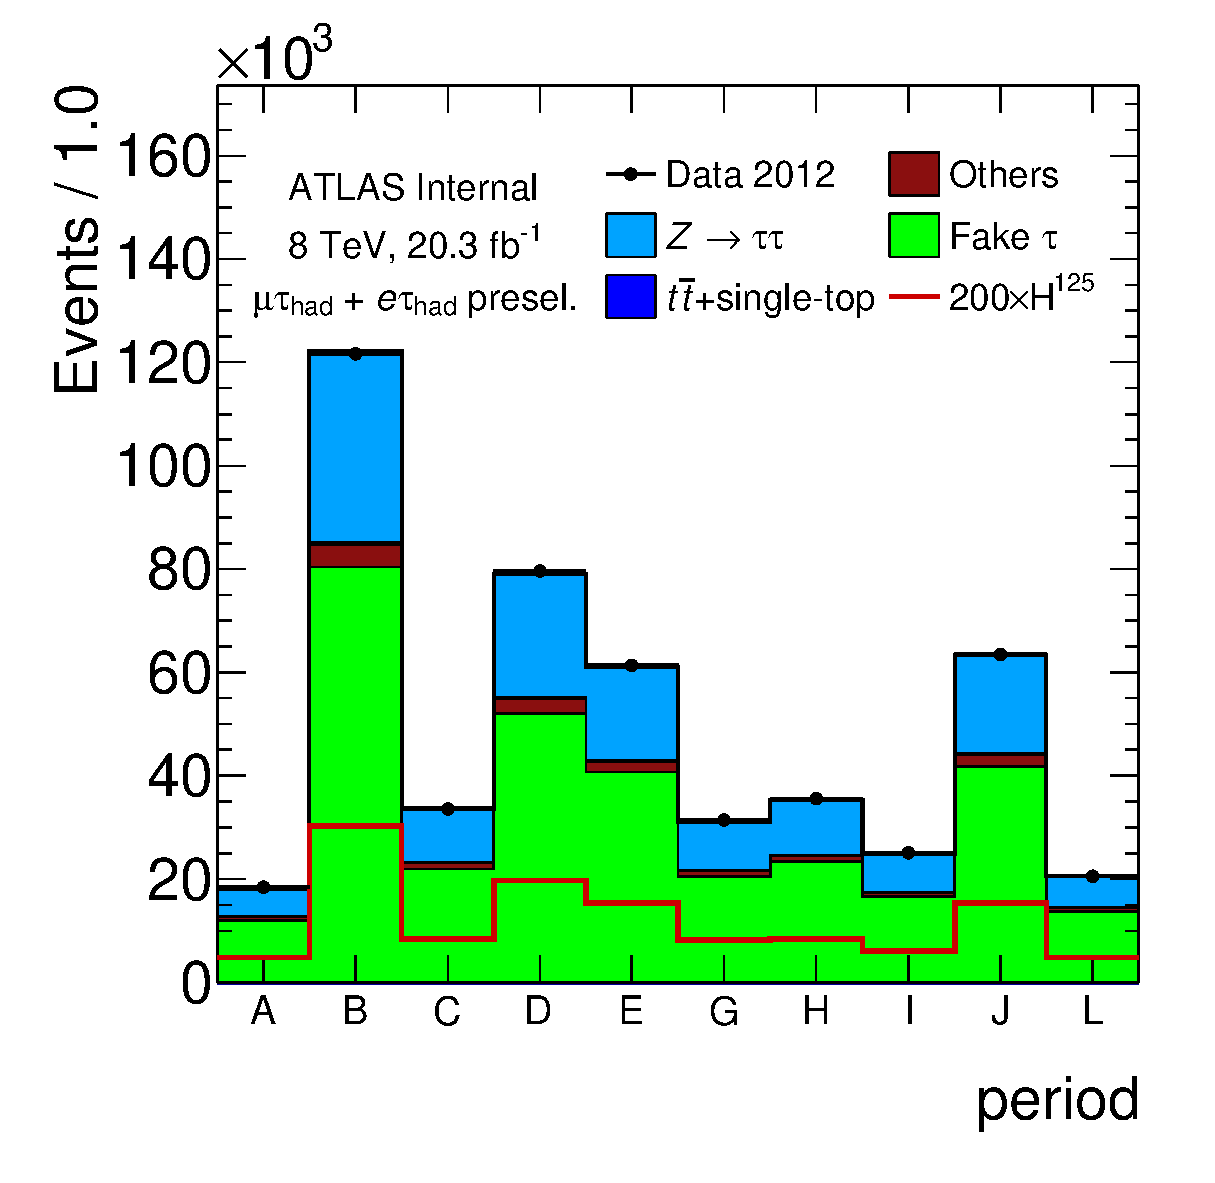
\includegraphics[width=0.32\textwidth]{figures/presel/period}
  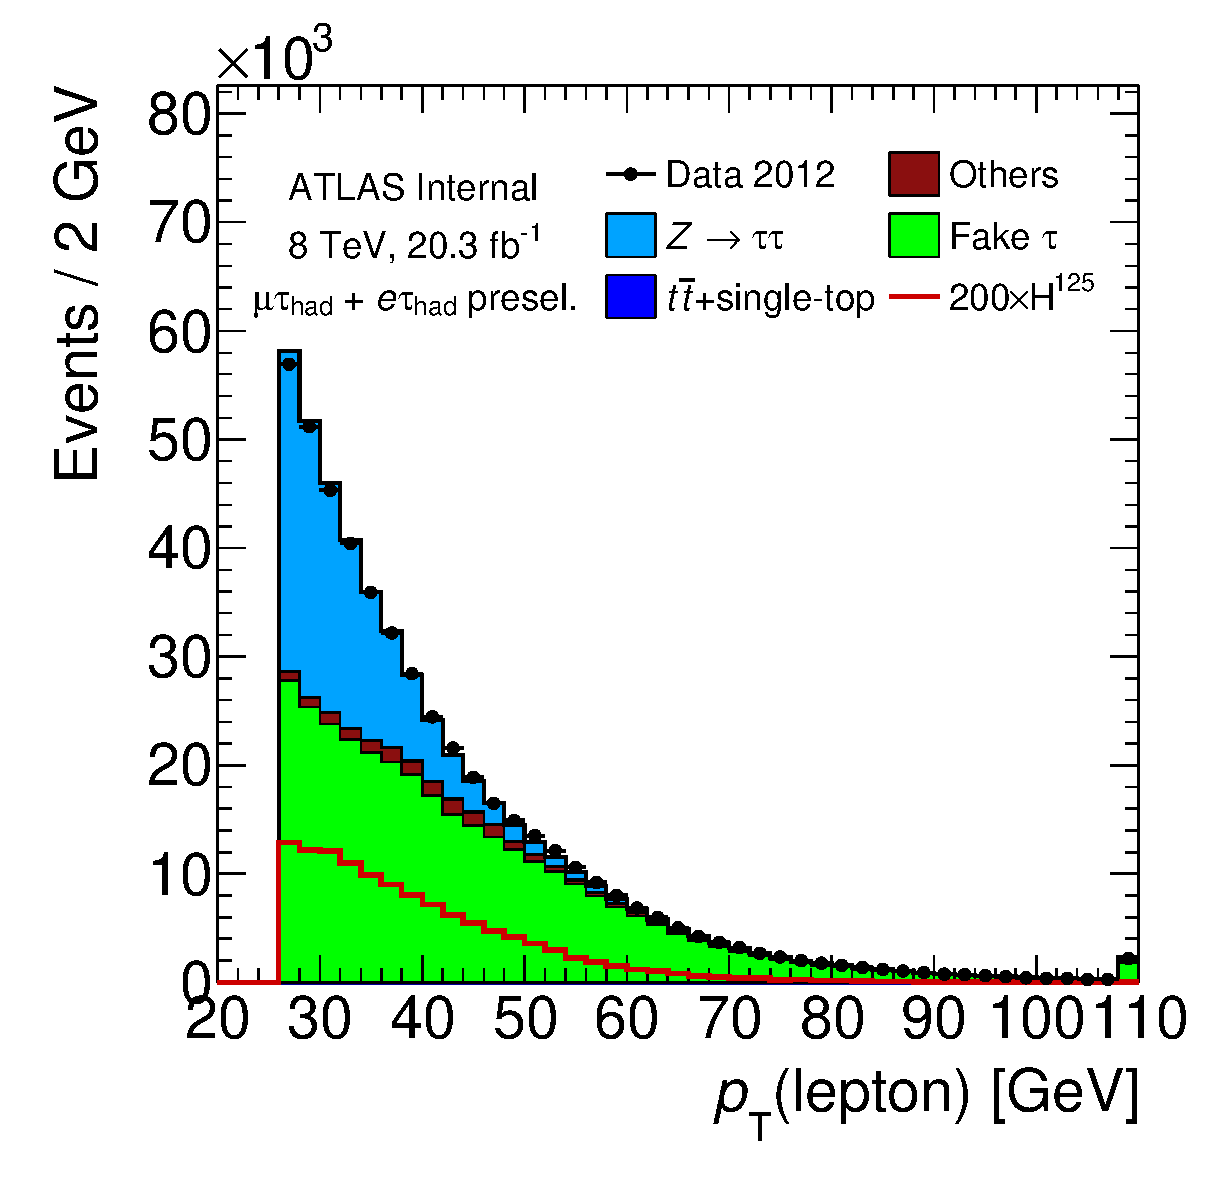
\includegraphics[width=0.32\textwidth]{figures/presel/lep-pt-hi}
  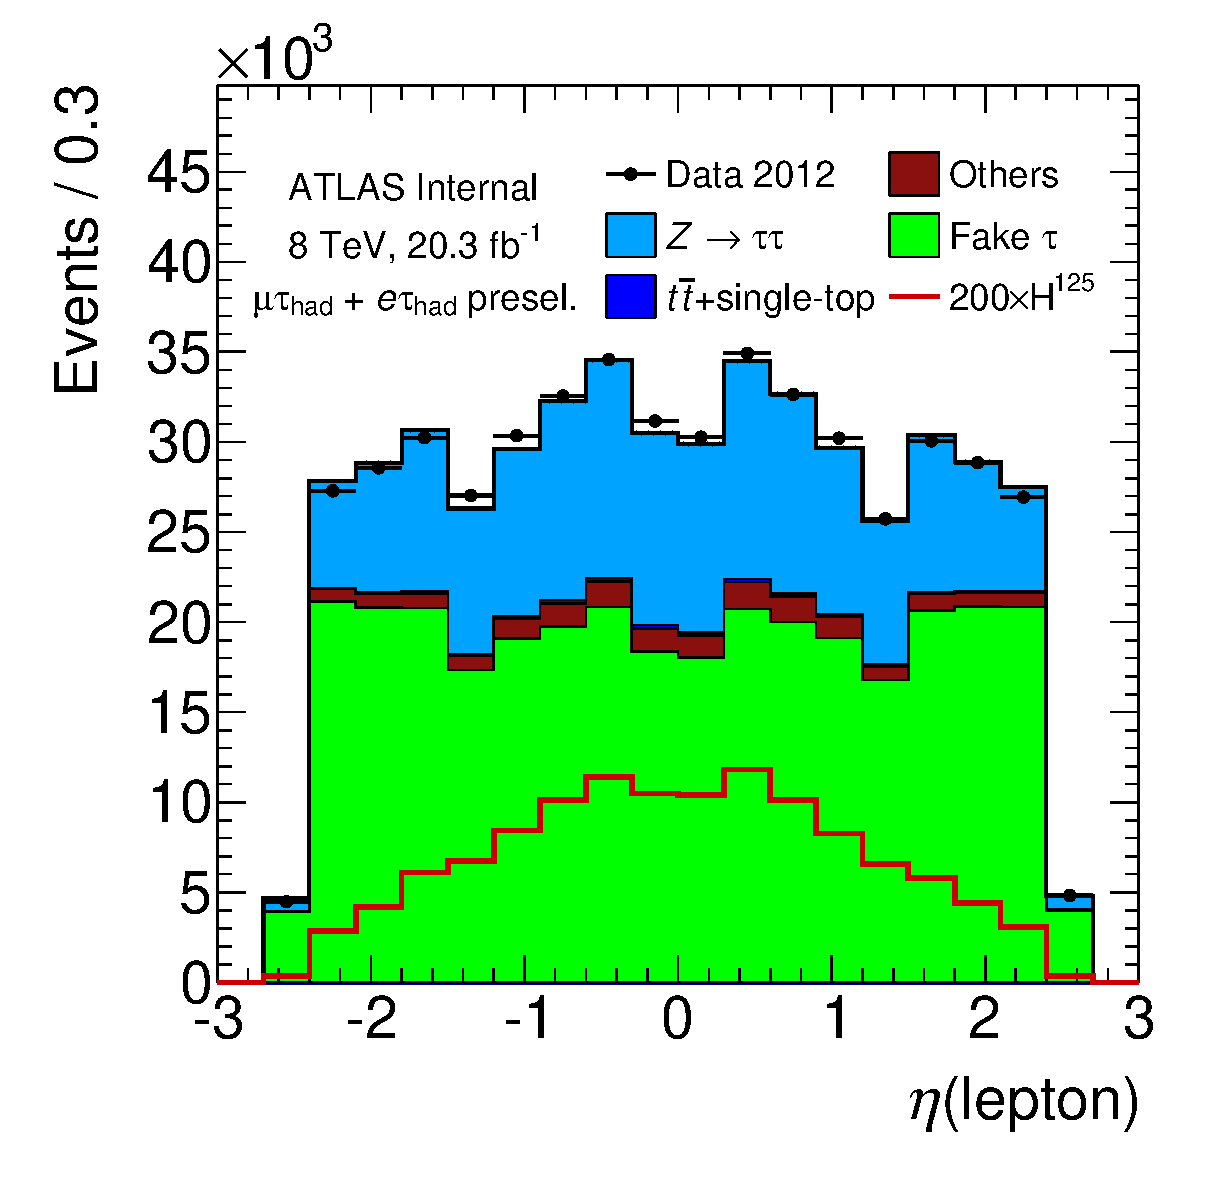
\includegraphics[width=0.32\textwidth]{figures/presel/lep-eta} \\
  % --------------
  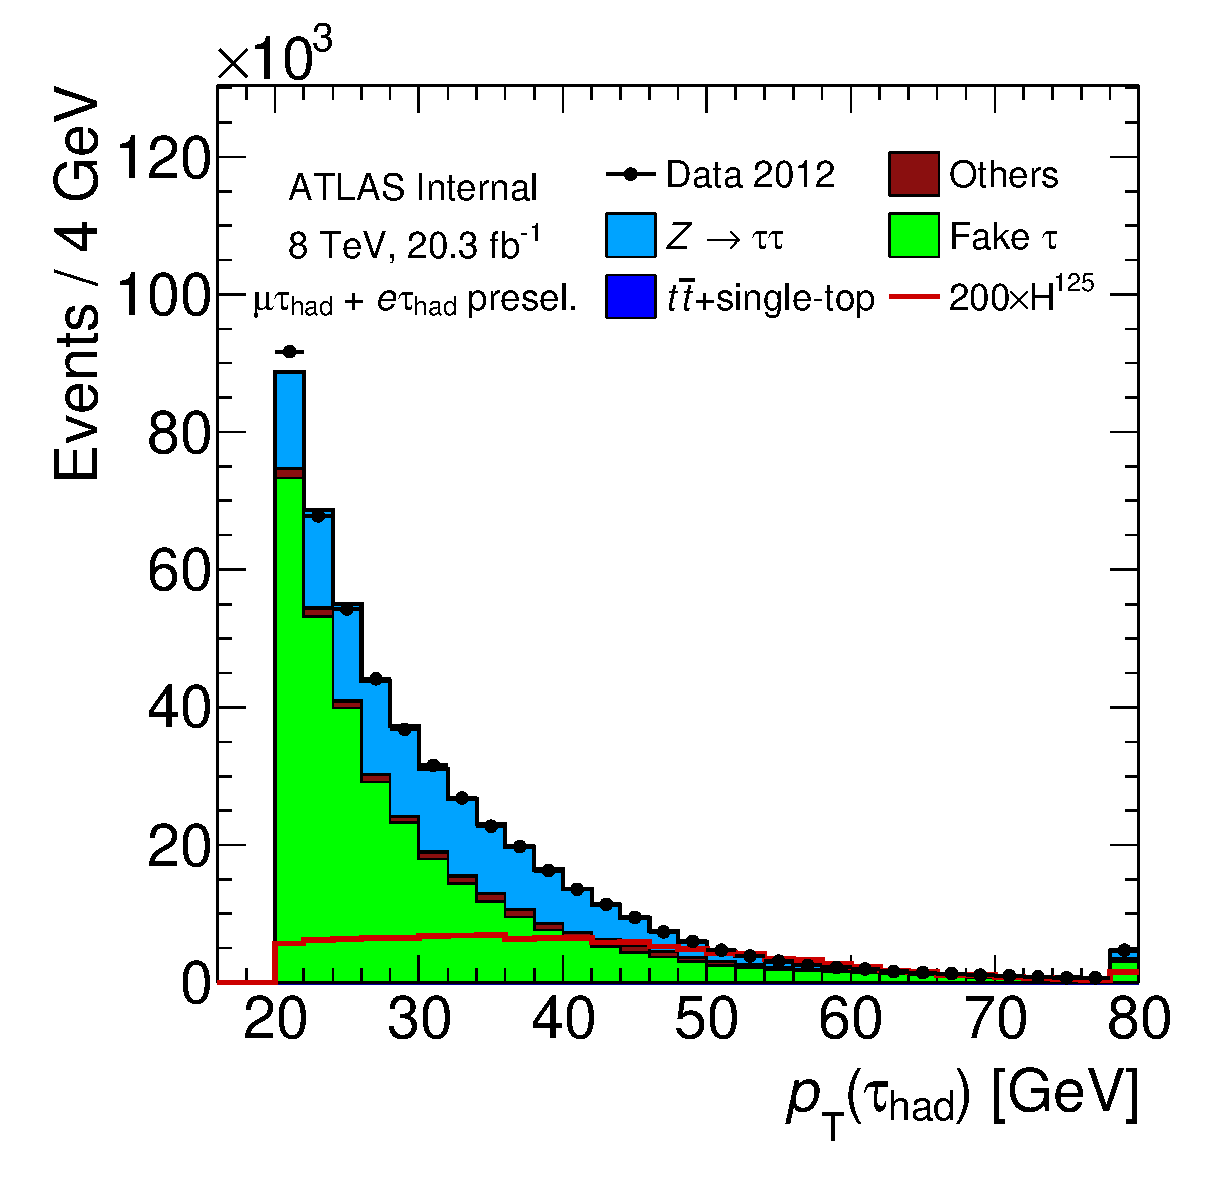
\includegraphics[width=0.32\textwidth]{figures/presel/tau-pt}
  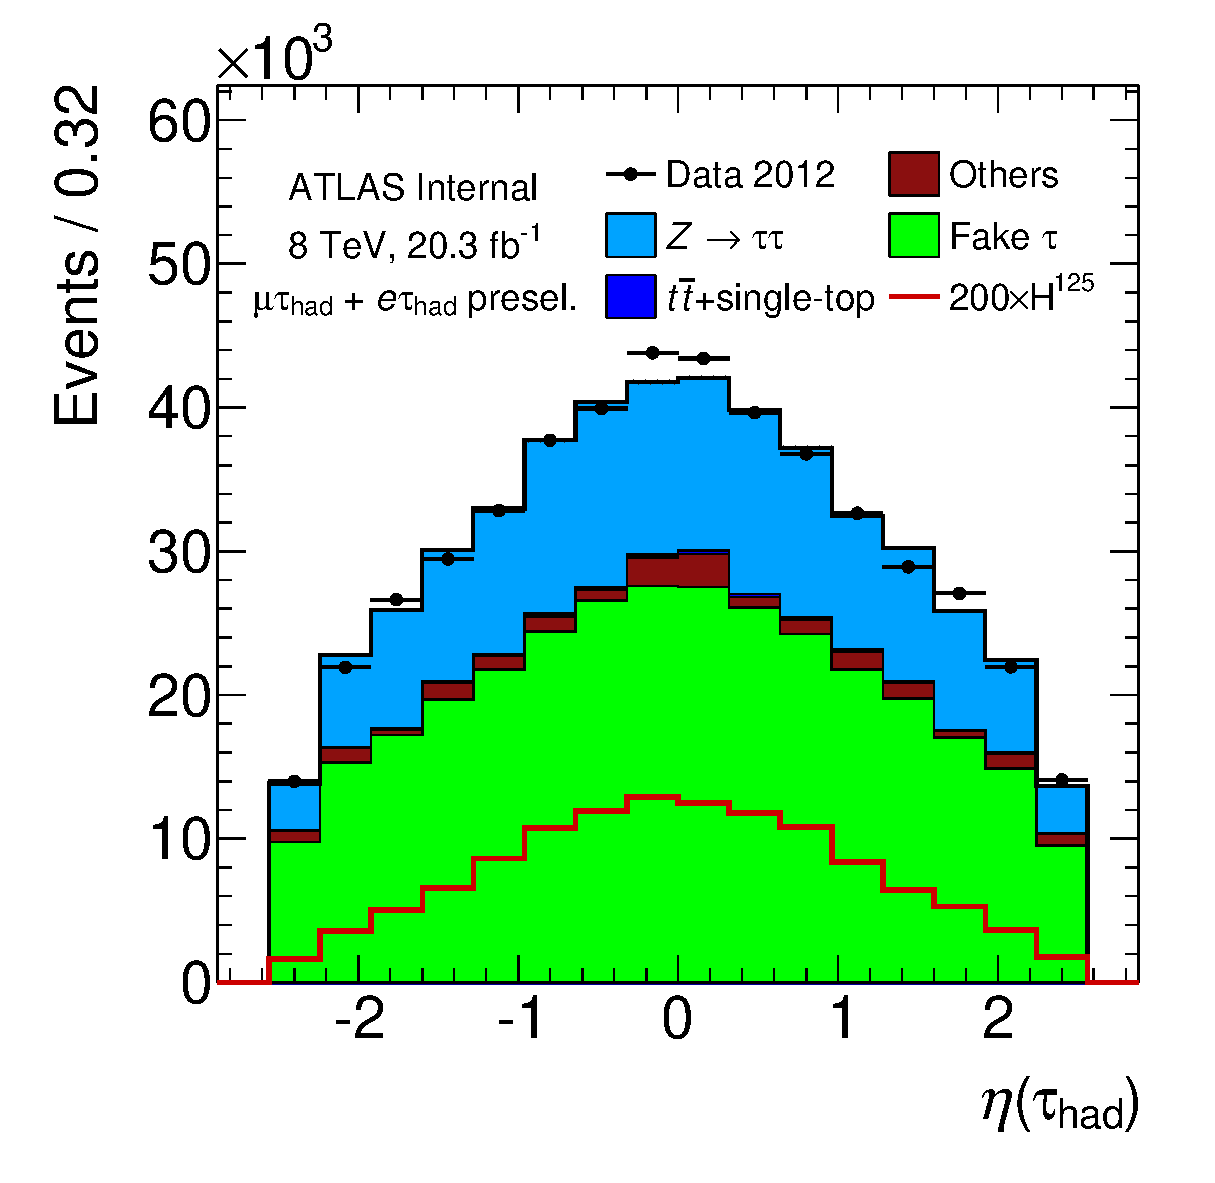
\includegraphics[width=0.32\textwidth]{figures/presel/tau-eta}
  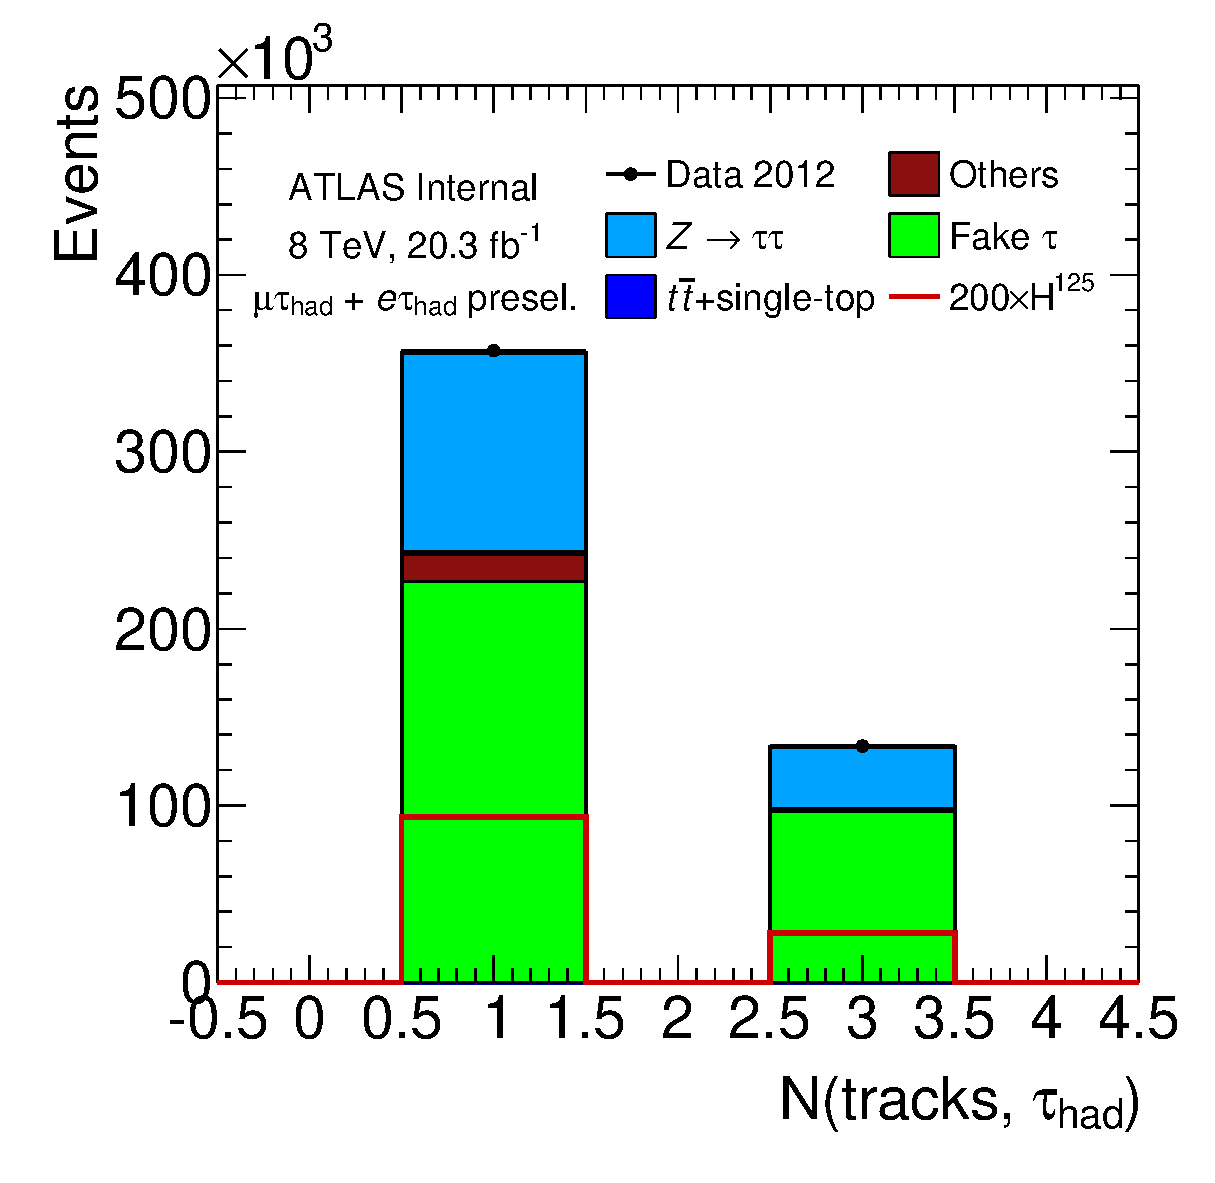
\includegraphics[width=0.32\textwidth]{figures/presel/tau-numTrack} \\
  % --------------
  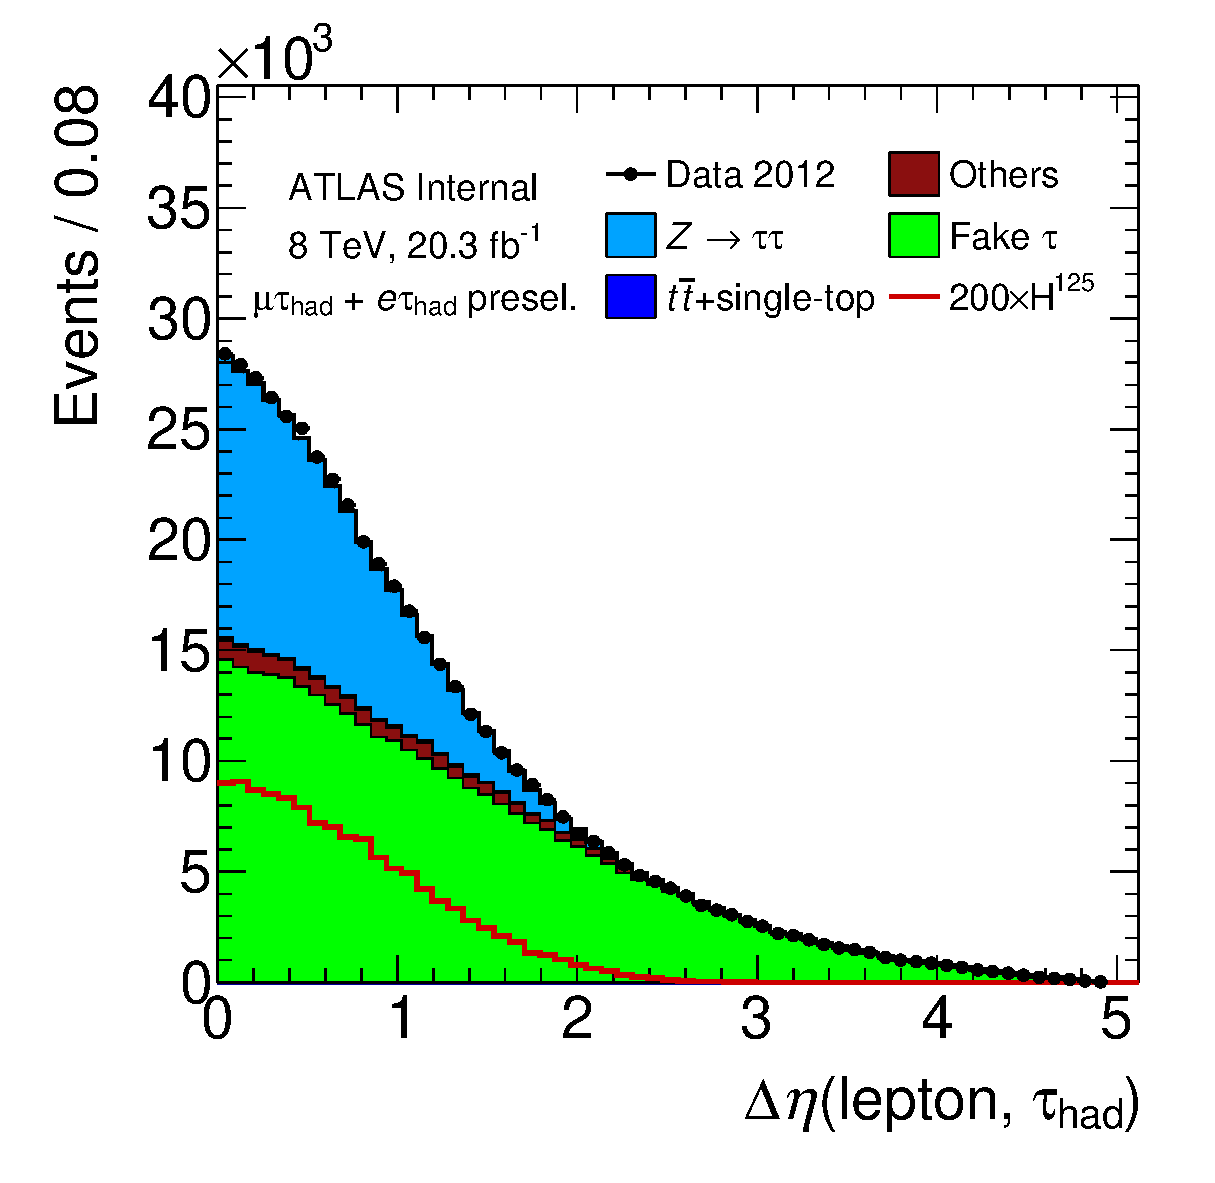
\includegraphics[width=0.32\textwidth]{figures/presel/taulep-deta}
  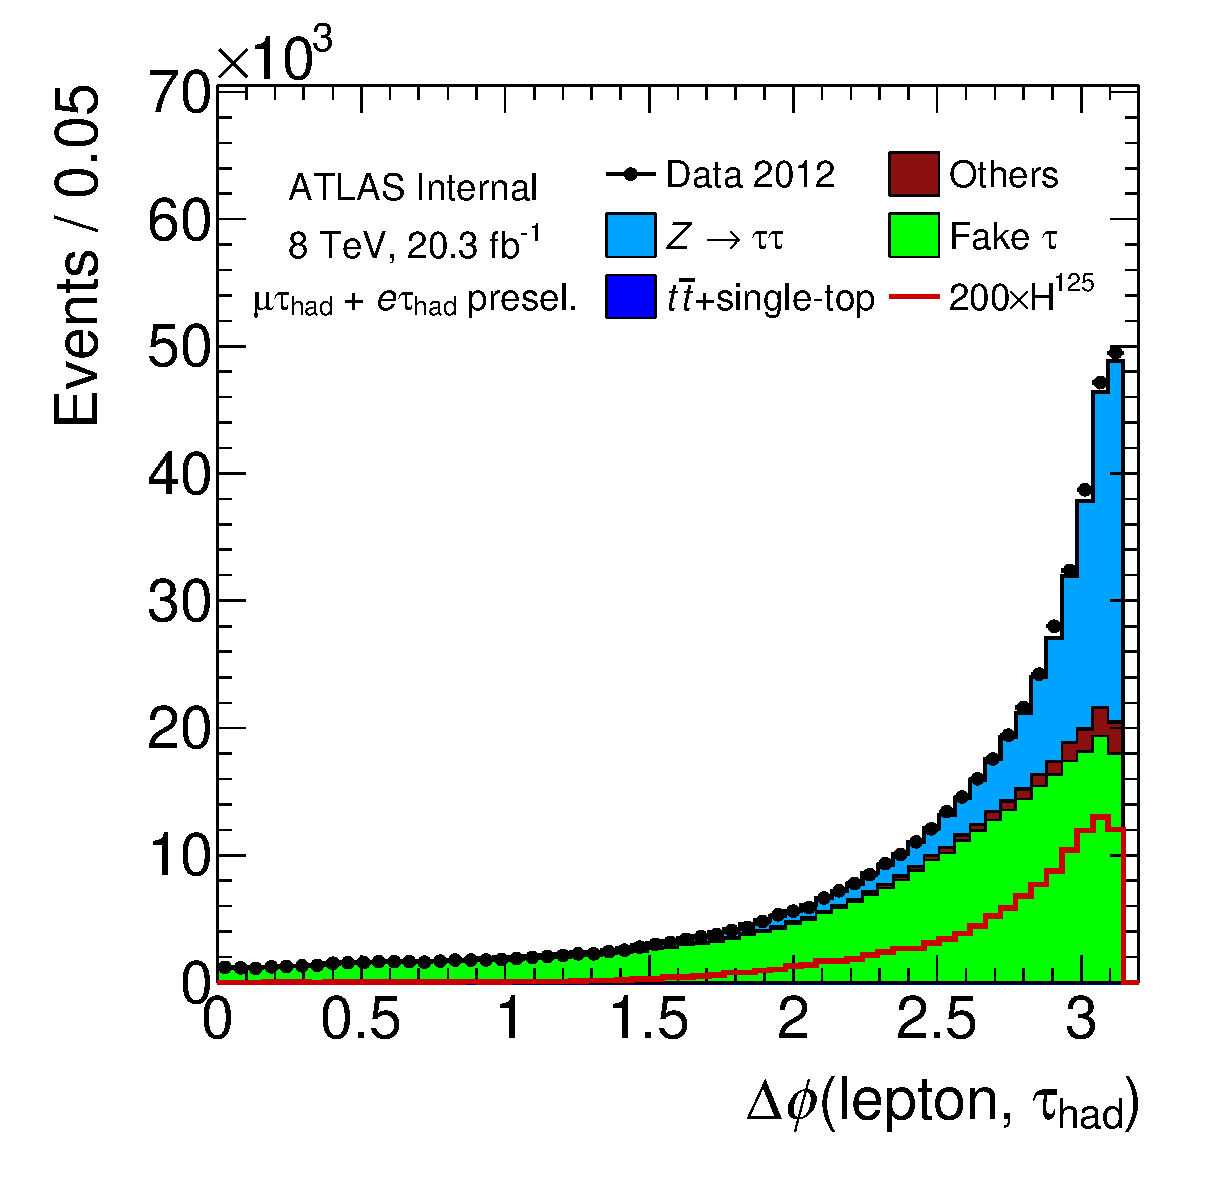
\includegraphics[width=0.32\textwidth]{figures/presel/taulep-dphi}
  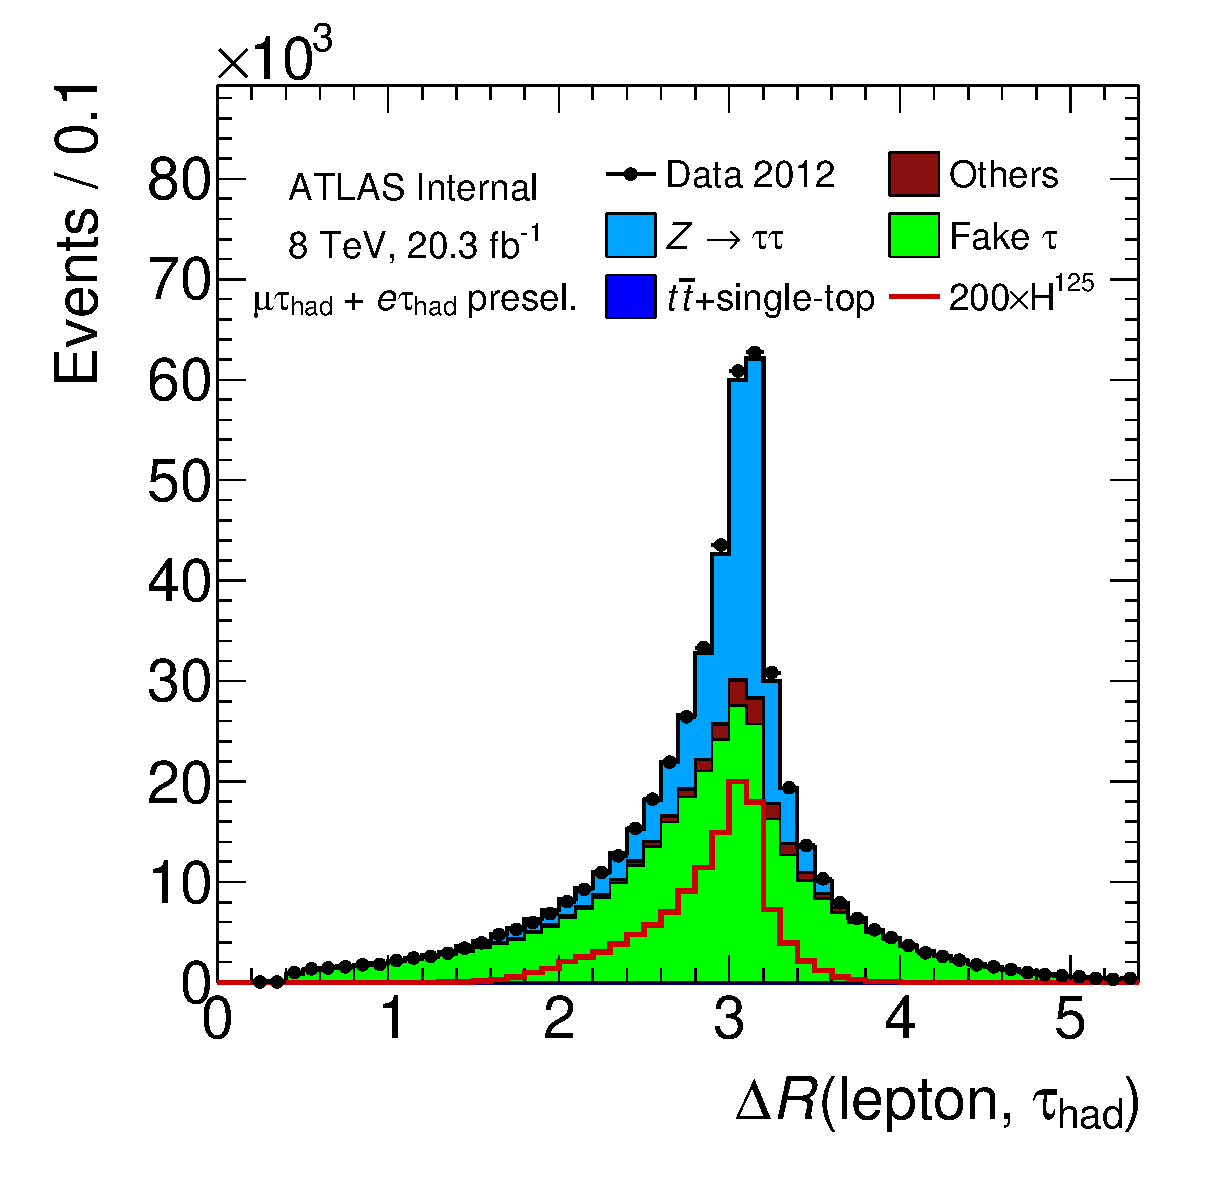
\includegraphics[width=0.32\textwidth]{figures/presel/taulep-dR} \\
  \caption{Kinematic distributions in the pre-selection category of the 8 TeV $\Htautaulh$ analysis.}
  \label{fig:stategy-presel-1}
\end{figure}

\clearpage

\begin{figure}[tp]
  \centering
  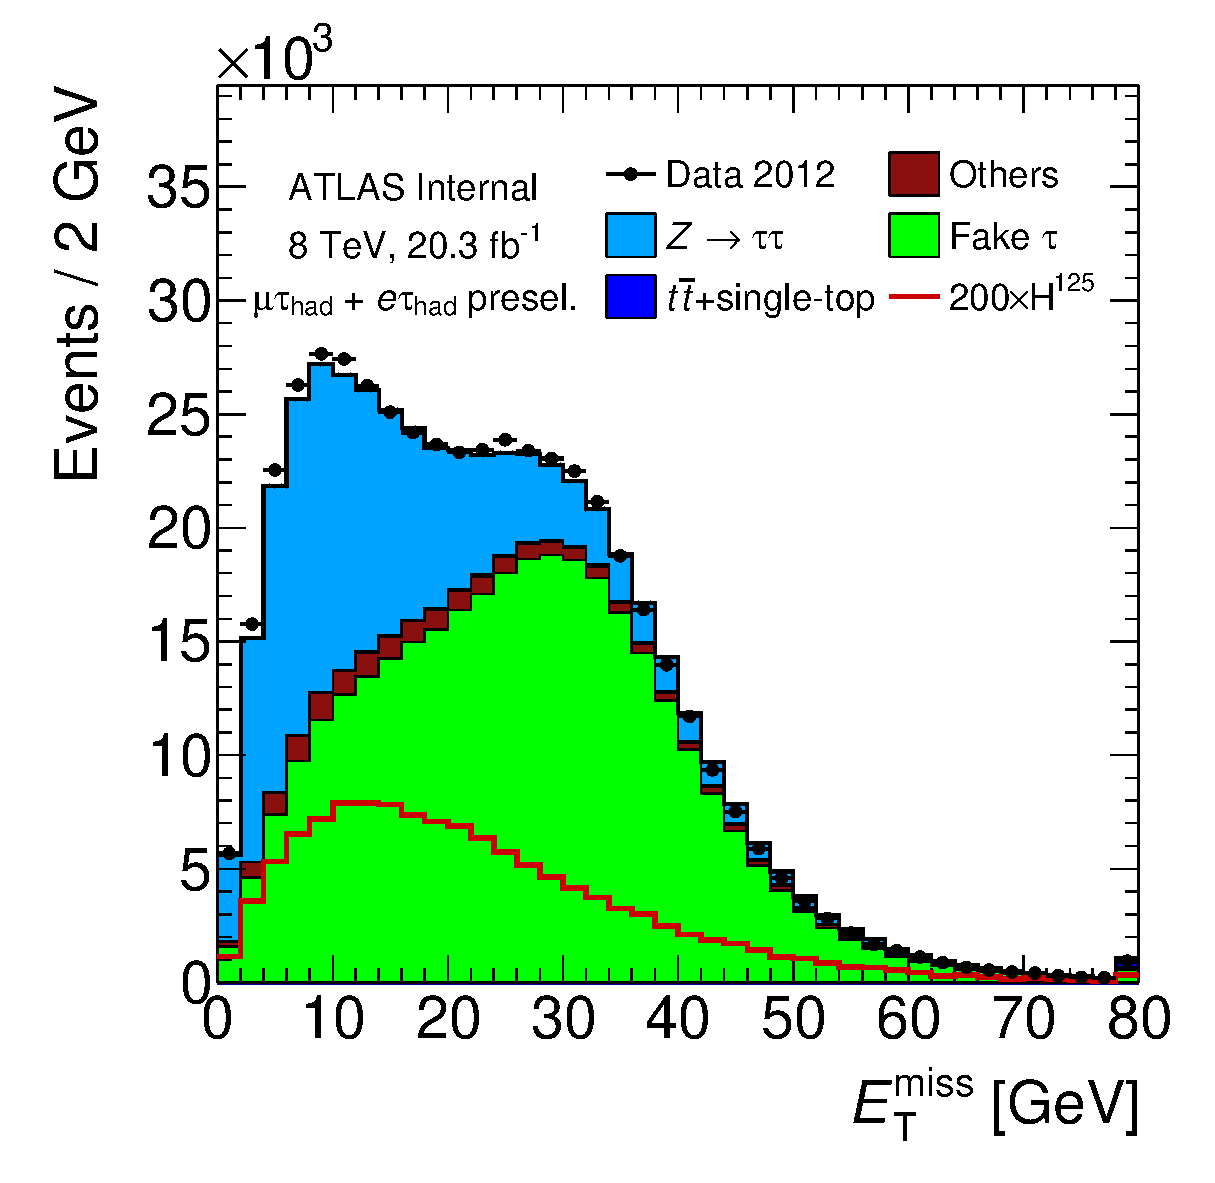
\includegraphics[width=0.32\textwidth]{figures/presel/met-pt}
  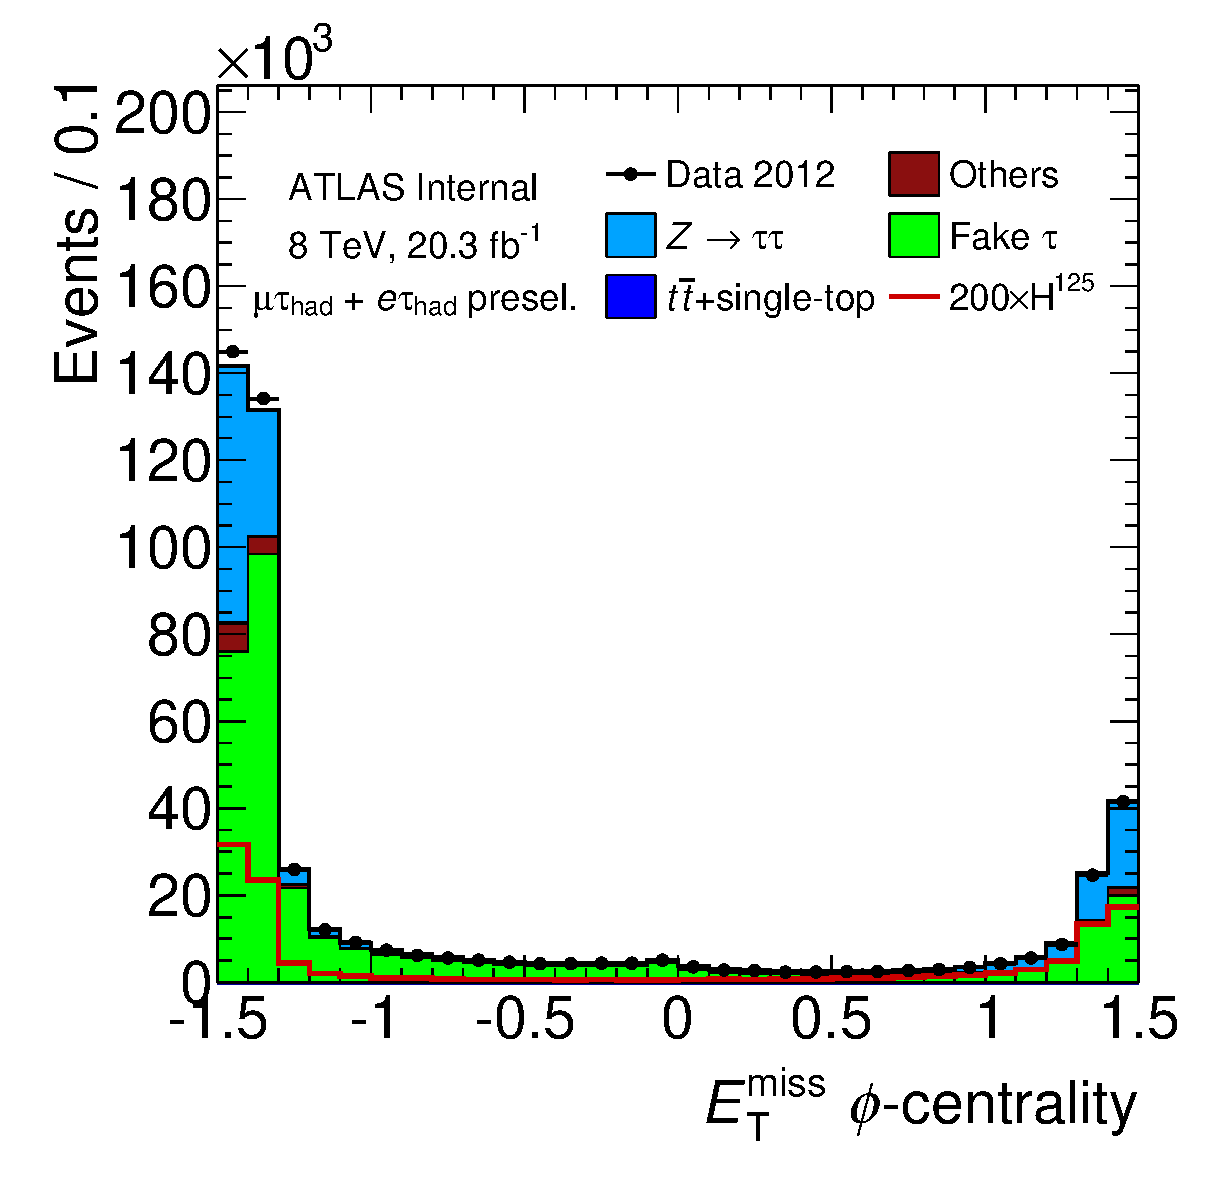
\includegraphics[width=0.32\textwidth]{figures/presel/met-phi-centrality}
  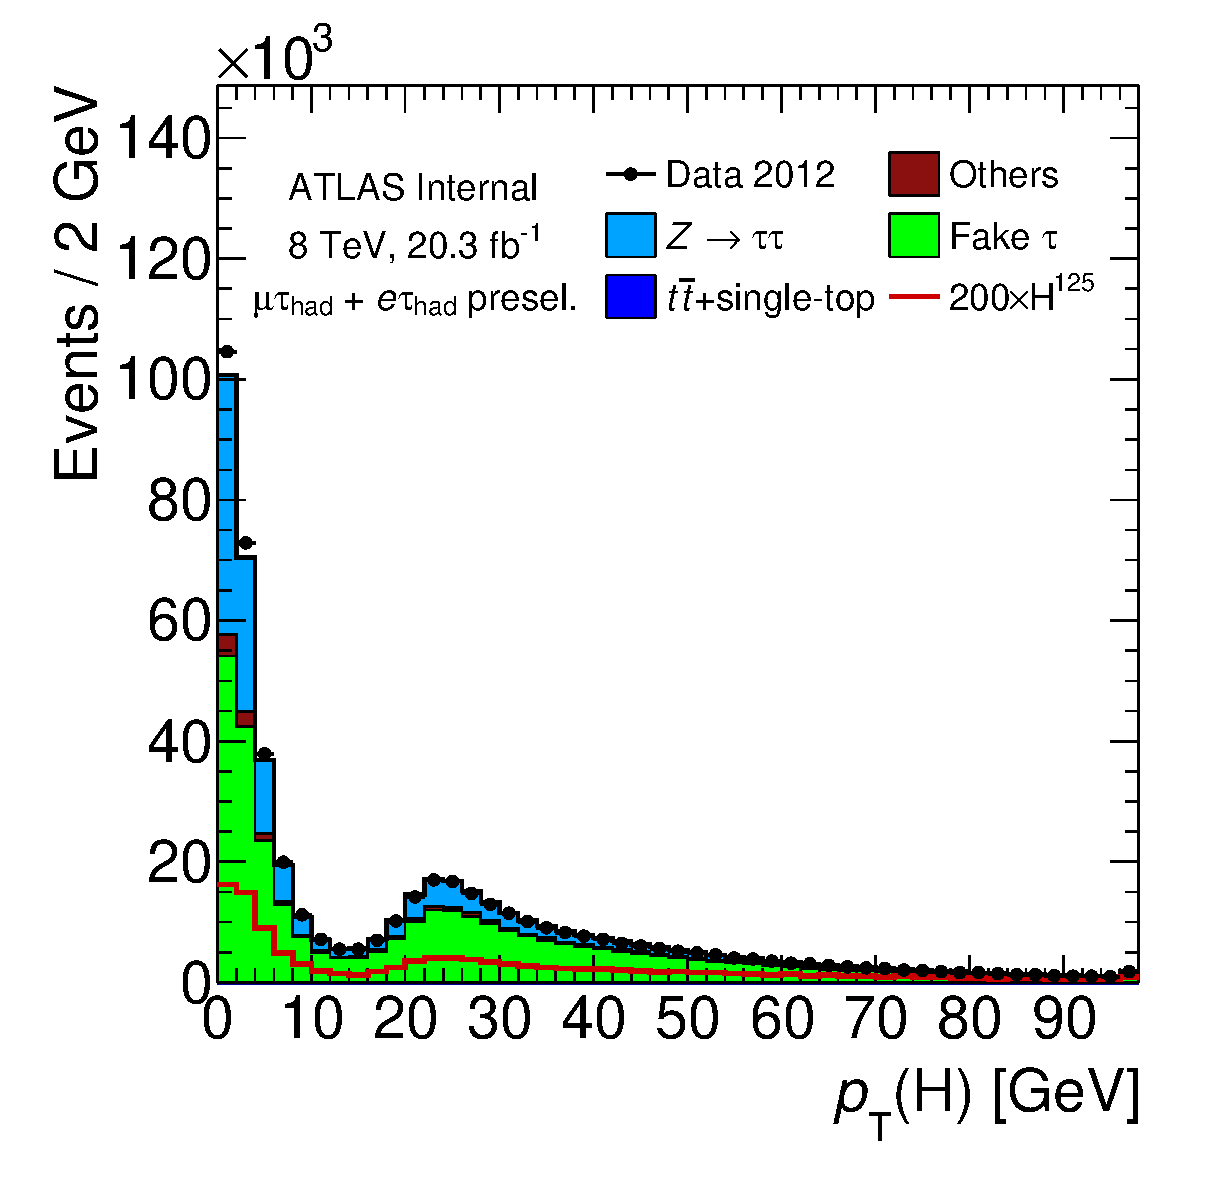
\includegraphics[width=0.32\textwidth]{figures/presel/H-pt} \\
  % --------------
  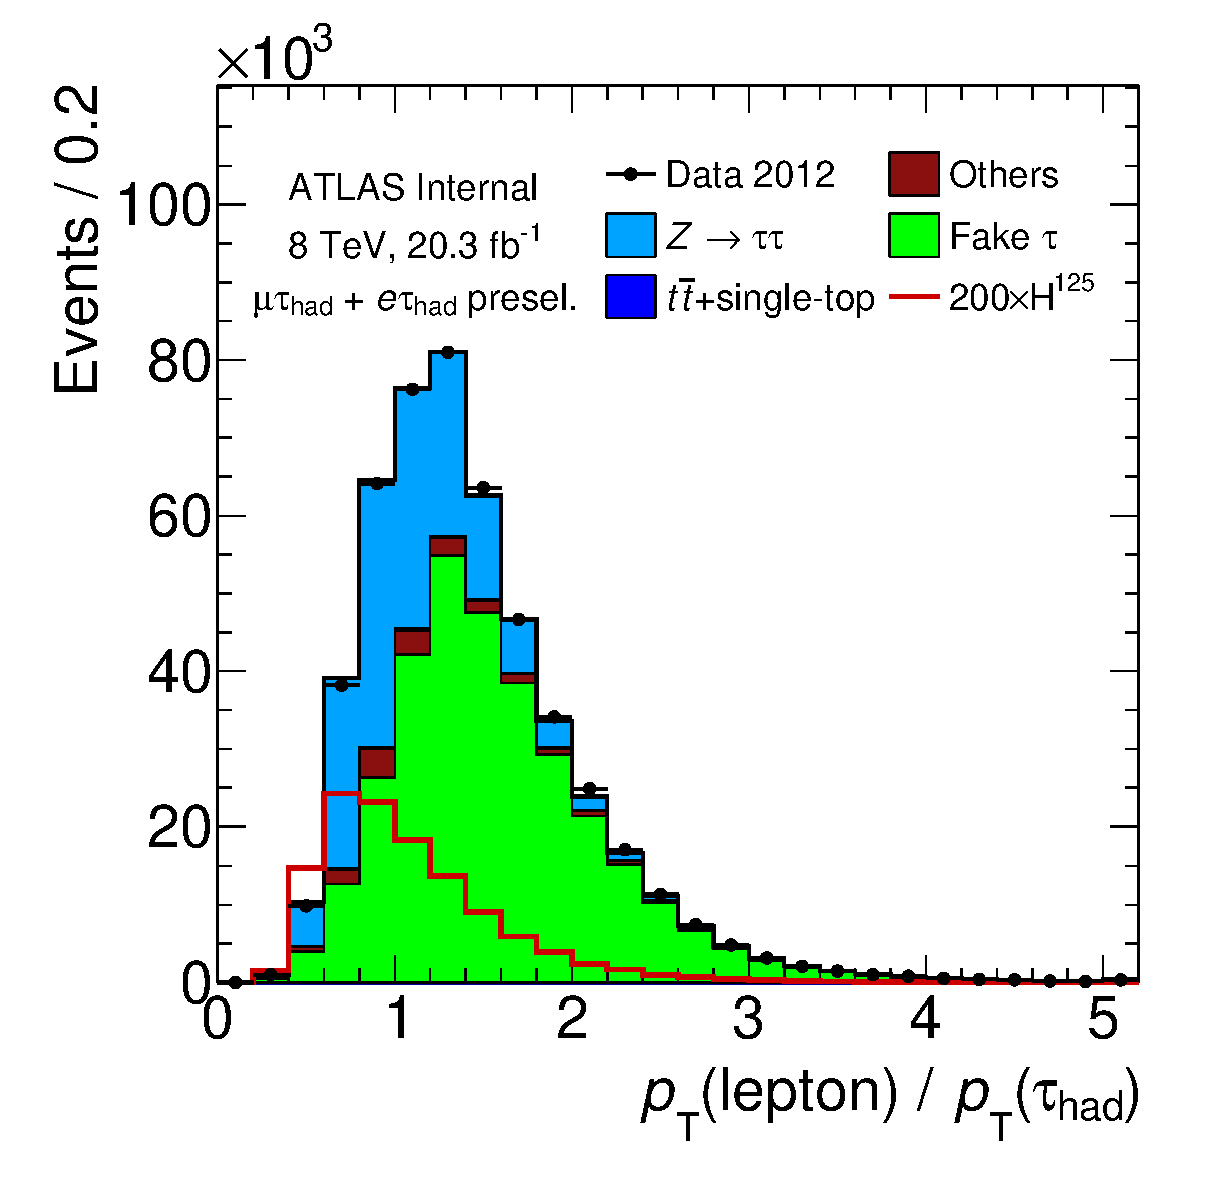
\includegraphics[width=0.32\textwidth]{figures/presel/taulep-ptratio}
  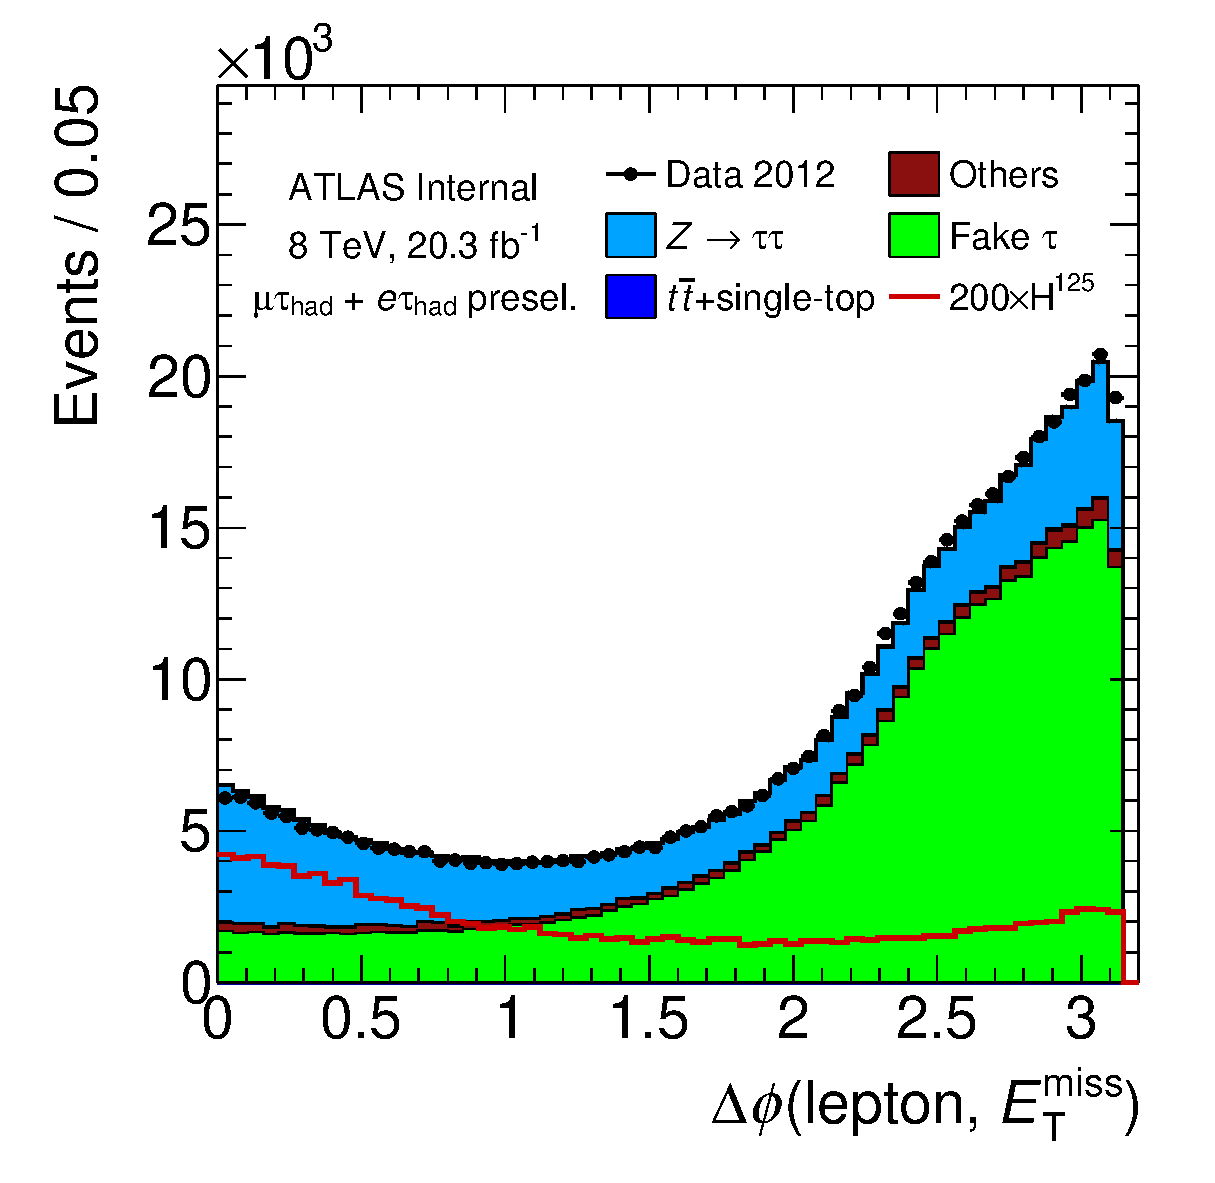
\includegraphics[width=0.32\textwidth]{figures/presel/lepmet-dphi}
  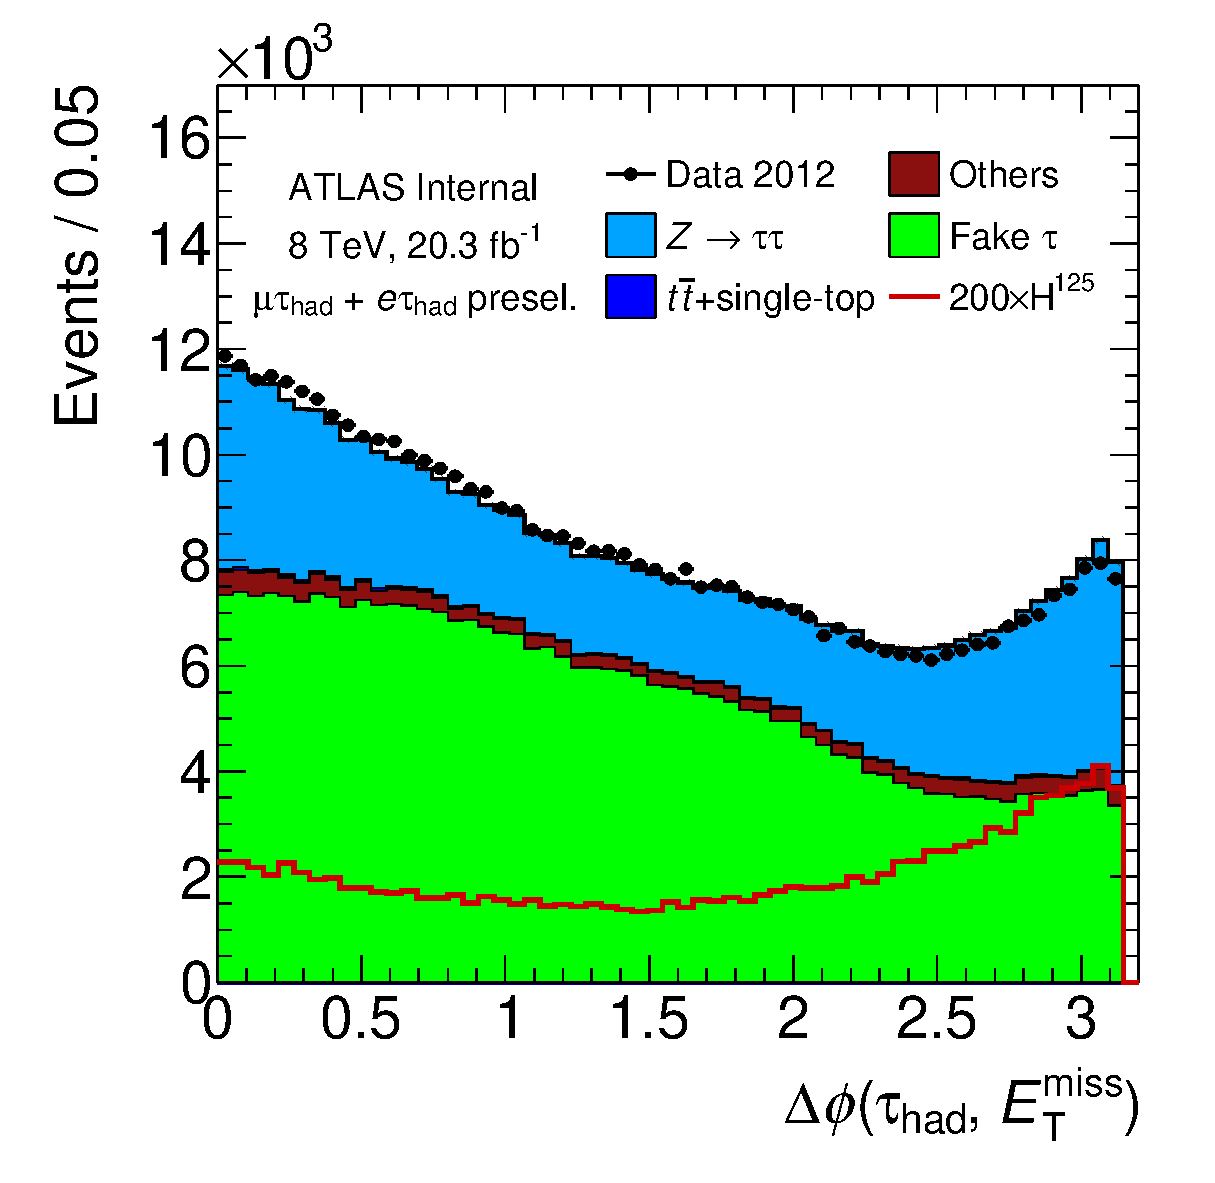
\includegraphics[width=0.32\textwidth]{figures/presel/taumet-dphi} \\
  % --------------
  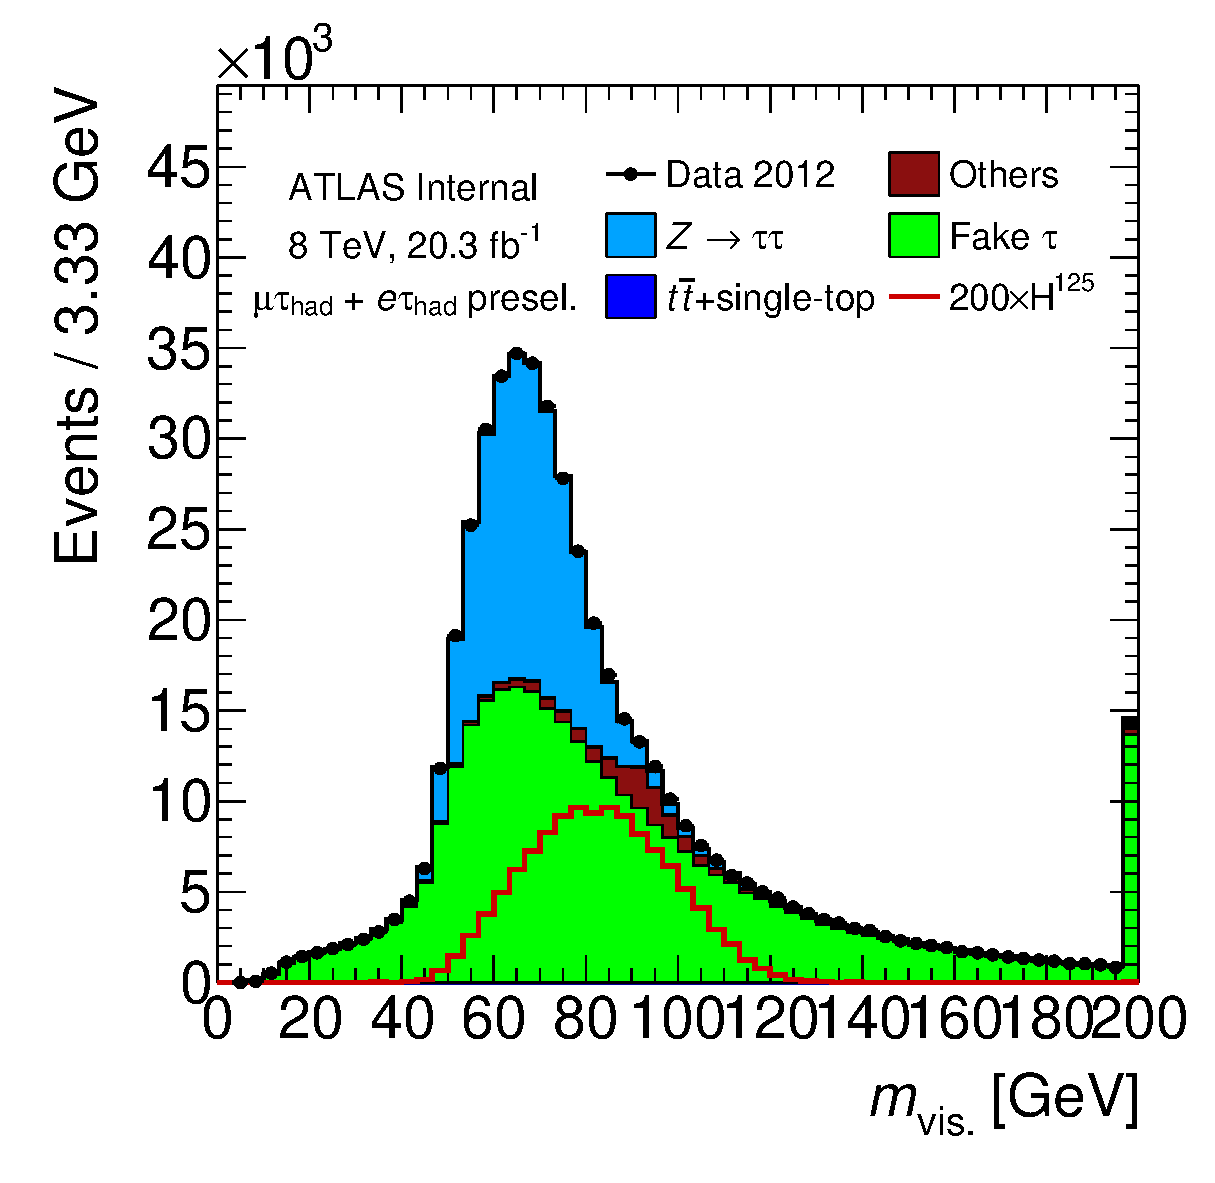
\includegraphics[width=0.32\textwidth]{figures/presel/mvis}
  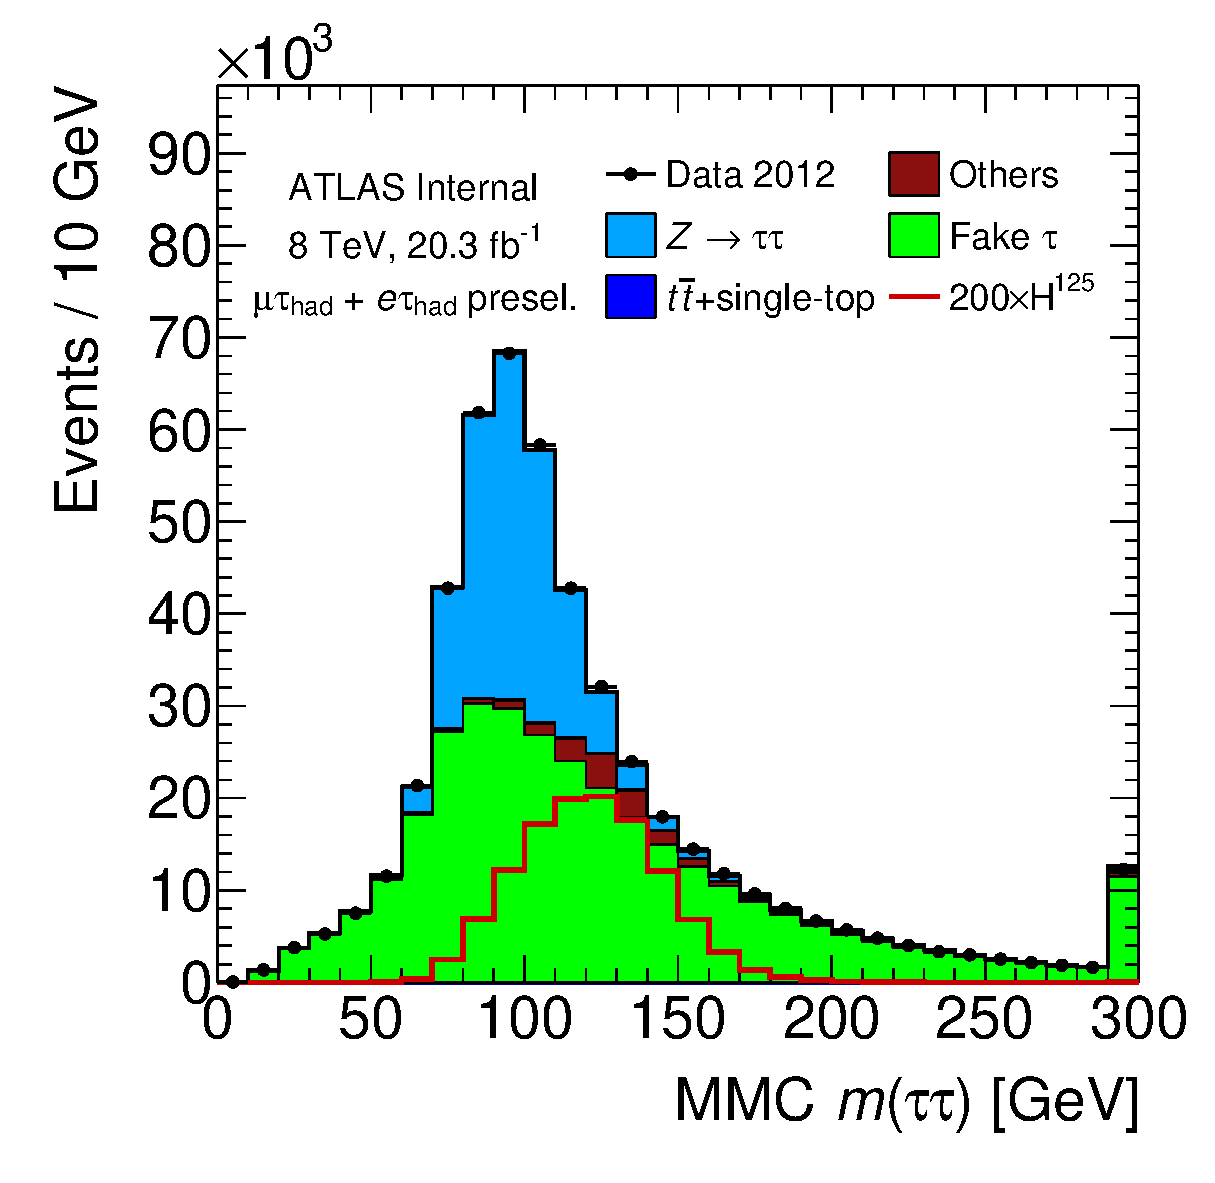
\includegraphics[width=0.32\textwidth]{figures/presel/mMMC}
  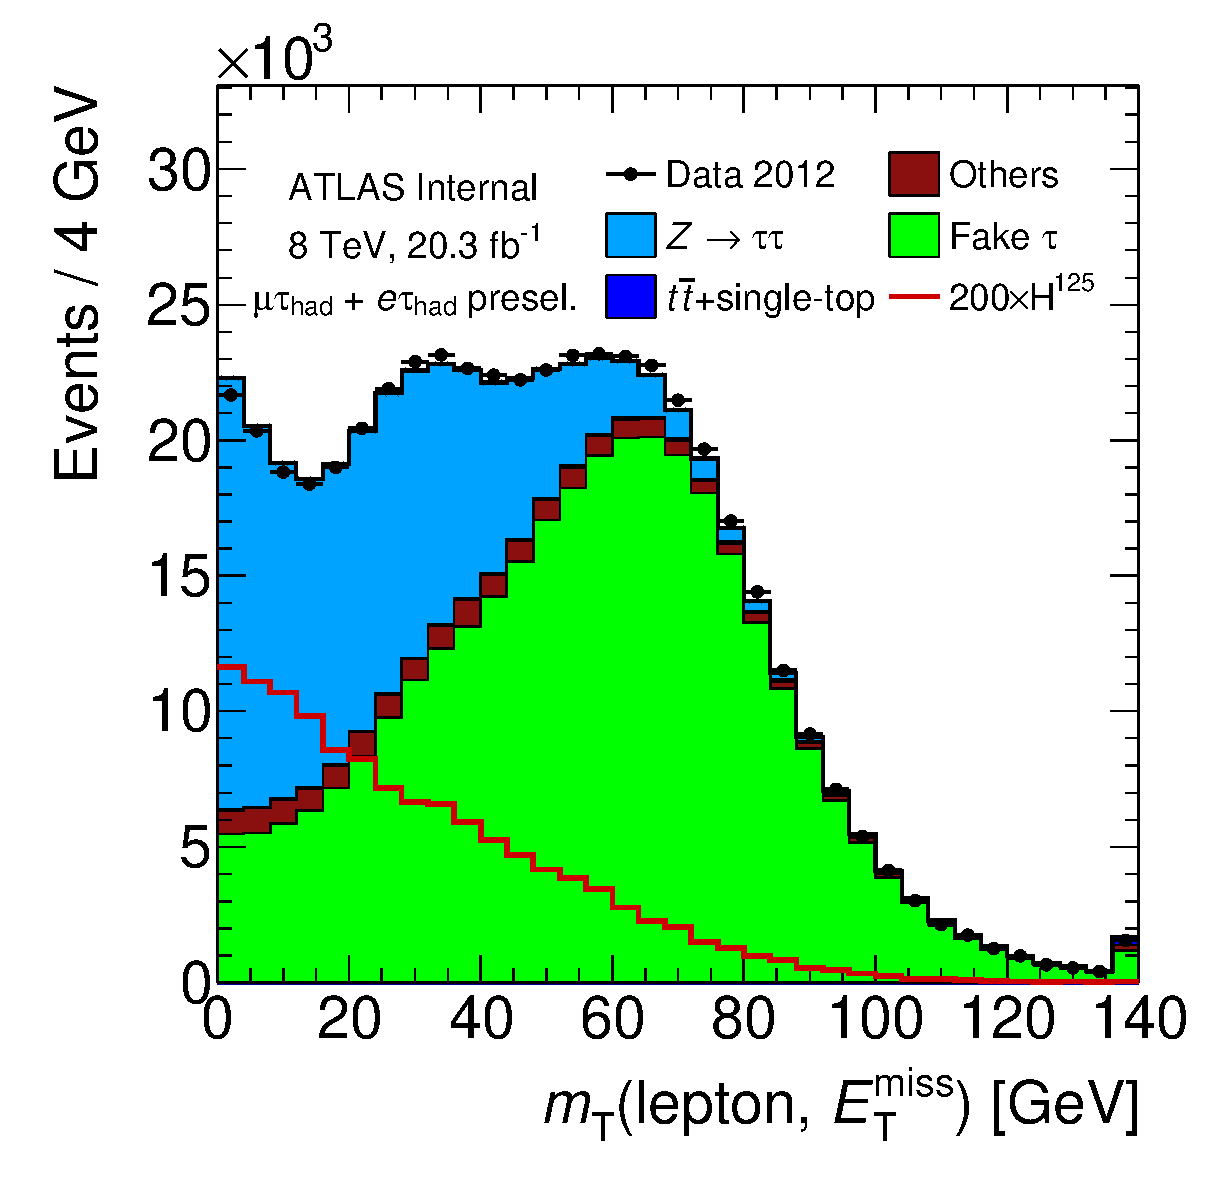
\includegraphics[width=0.32\textwidth]{figures/presel/mT-hi} \\
  % --------------
  \caption{Kinematic distributions in the pre-selection category of the 8 TeV $\Htautaulh$ analysis.}
  \label{fig:stategy-presel-2}
\end{figure}

\subsection{VBF category}
\label{sec:strategy-VBF}

\subsection{Boosted category}
\label{sec:strategy-boost}

\clearpage

\section{$\tautau$ mass reconstruction}
\label{sec:strategy-mtautau}

\subsection{$\tau\tau$ systems}
\label{sec:strategy-mtautau-intro}

\subsection{$\mMMC$ algorithm}
\label{sec:strategy-mtautau-mMMC}

% MMC cartoon
% ---------------------------------------------------------------------------------
\begin{figure}[tp]
  \centering
  \includegraphics[width=0.90\textwidth]{figures/mtautau/mmc-cartoon}
  \caption{Cartoon of the $\mMMC$ reconstruction algorithm. Black, filled lines indicate items measured directly ($\ell$, $\tauh$). Red, dotted lines indicate items which cannot be measured (neutrinos). The black, dashed line indicates the $\MET$, which is measured indirectly. Blue indicates items which the $\mMMC$ scans to find an optimal solution ($\Delta\phi$, $\MET$).}
  \label{fig:strategy-mtautau-cartoon}
\end{figure}

% MMC input assumptions
% ---------------------------------------------------------------------------------
\begin{figure}[tp]
  \centering
  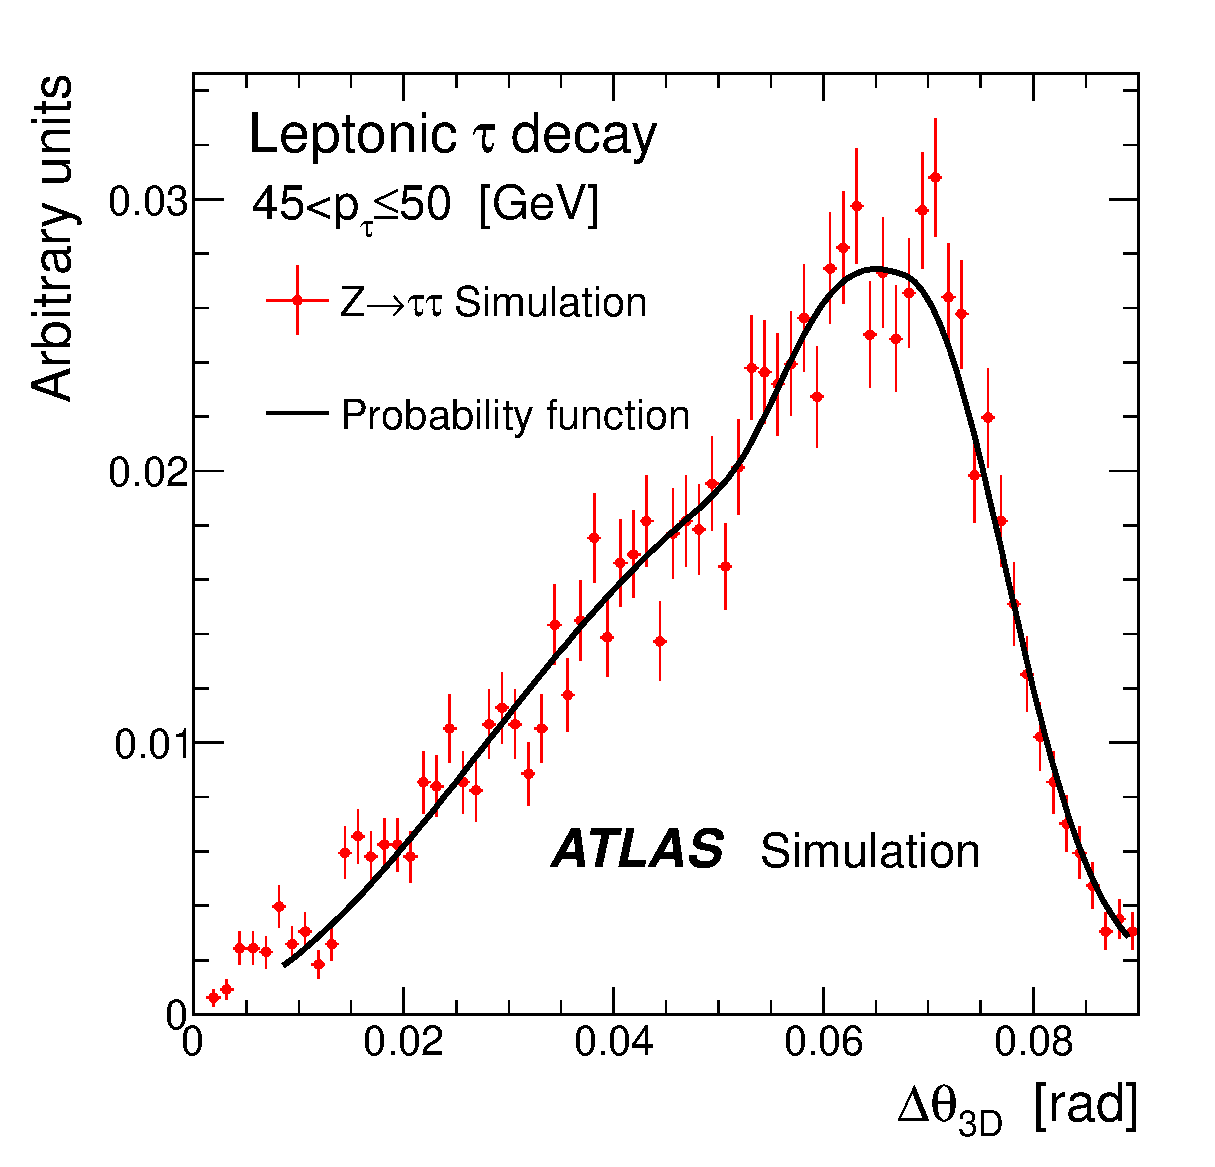
\includegraphics[width=0.32\textwidth]{figures/ATLAS-CONF-2011-132/fig_01a}
  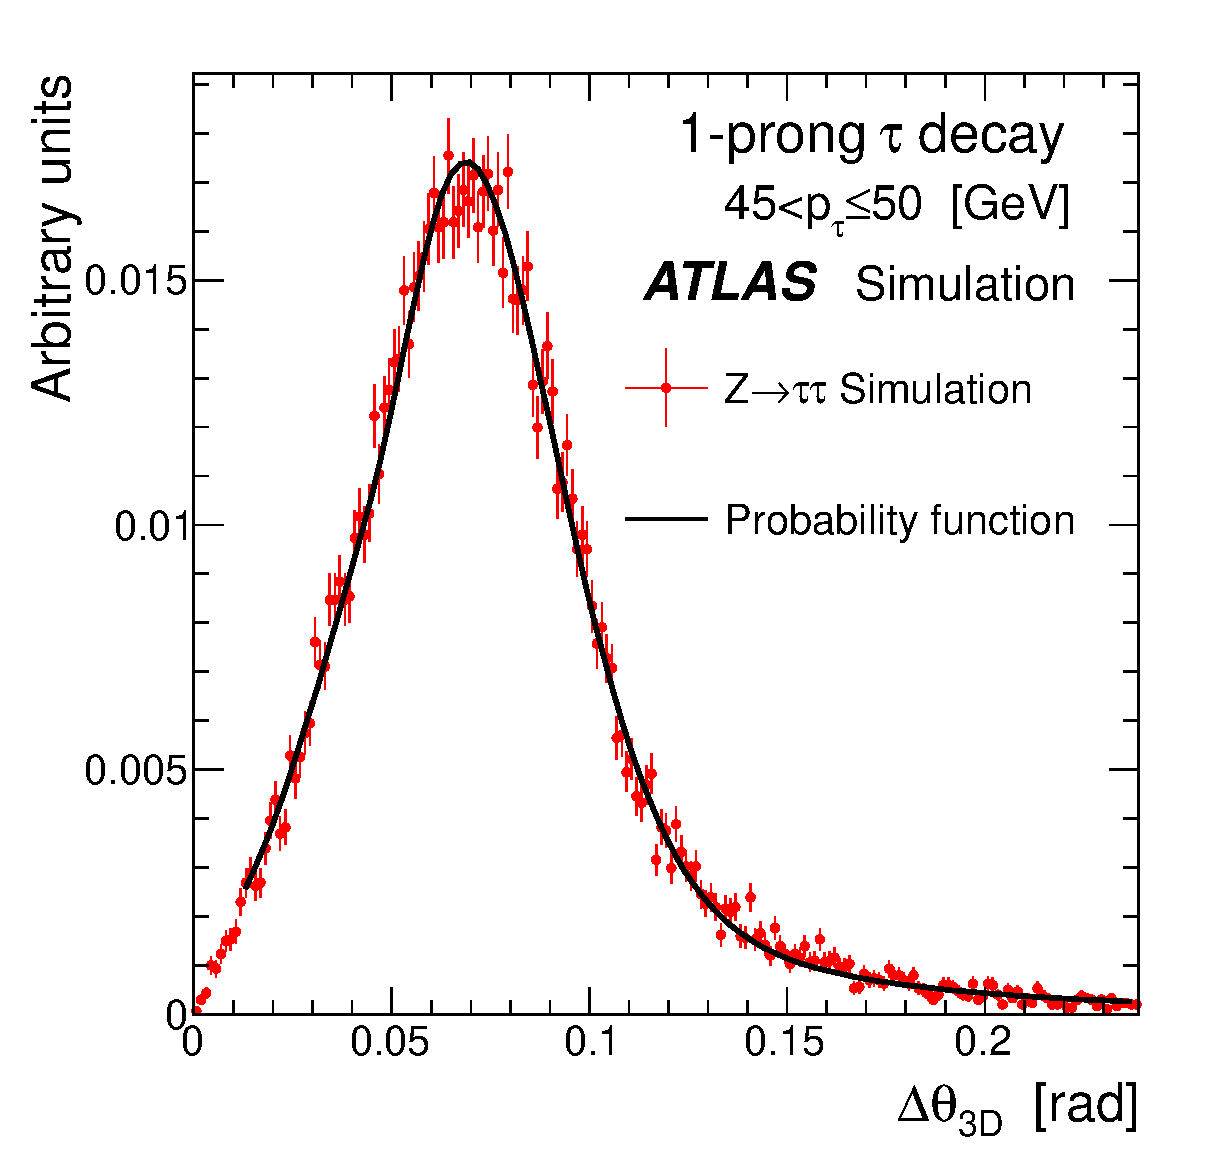
\includegraphics[width=0.32\textwidth]{figures/ATLAS-CONF-2011-132/fig_01b}
  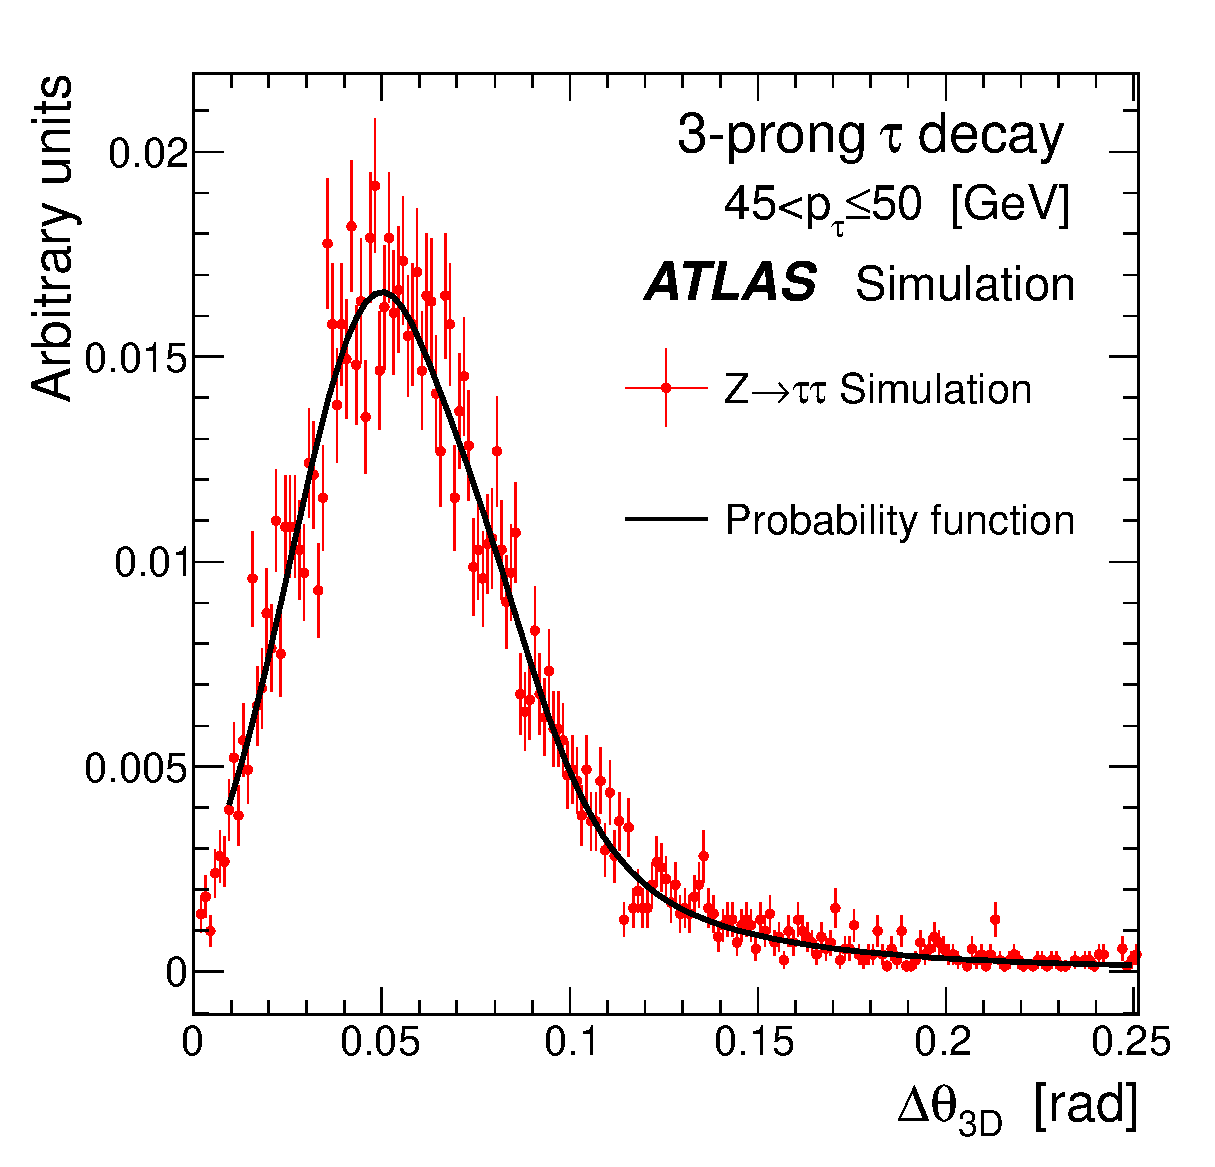
\includegraphics[width=0.32\textwidth]{figures/ATLAS-CONF-2011-132/fig_01c}
  \caption{Input assumptions of the three-dimensional angle between the visible and invisible tau lepton decay products, for leptonic decays (left), 1-track hadronic decays (center), and 3-track hadronic decays (right)~\cite{ATLAS-CONF-2011-132}.}
  \label{fig:strategy-mtautau-inputs}
\end{figure}

\subsection{Performance}
\label{sec:strategy-mtautau-performance}

% mass ROCs
% ---------------------------------------------------------------------------------
\begin{figure}[tp]
  \centering
  \includegraphics[width=0.48\textwidth]{figures/mtautau/mtautau-boost}
  \includegraphics[width=0.48\textwidth]{figures/mtautau/mtautau-vbf}
  \caption{Efficiency for $\Htautaulh$ versus the efficiency for $\Ztautaulh$ for various $\mtautau$ reconstruction algorithms in the boosted category (left) and VBF category (right).}
  \label{fig:strategy-mtautau-ROC}
\end{figure}
% ---------------------------------------------------------------------------------

\section{MVA discrimination}
\label{sec:strategy-mva}

\subsection{Inputs}
\label{sec:strategy-mva-inputs}

% centrality cartoons
% ---------------------------------------------------------------------------------
\begin{figure}[tp]
  \centering
  \includegraphics[width=0.48\textwidth]{figures/backgrounds/cartoon_lepton_eta_centrality}
  \includegraphics[width=0.48\textwidth]{figures/backgrounds/cartoon_met_phi_centrality}
  \caption{Cartoons of lepton $\eta$-centrality (left) and $\MET$ $\phi$-centrality (right), courtesy of Tae Min Hong.}
  \label{fig:strategy-centrality-cartoons}
\end{figure}

% boost
% ---------------------------------------------------------------------------------
\clearpage
\begin{figure}[tp]
  \centering
  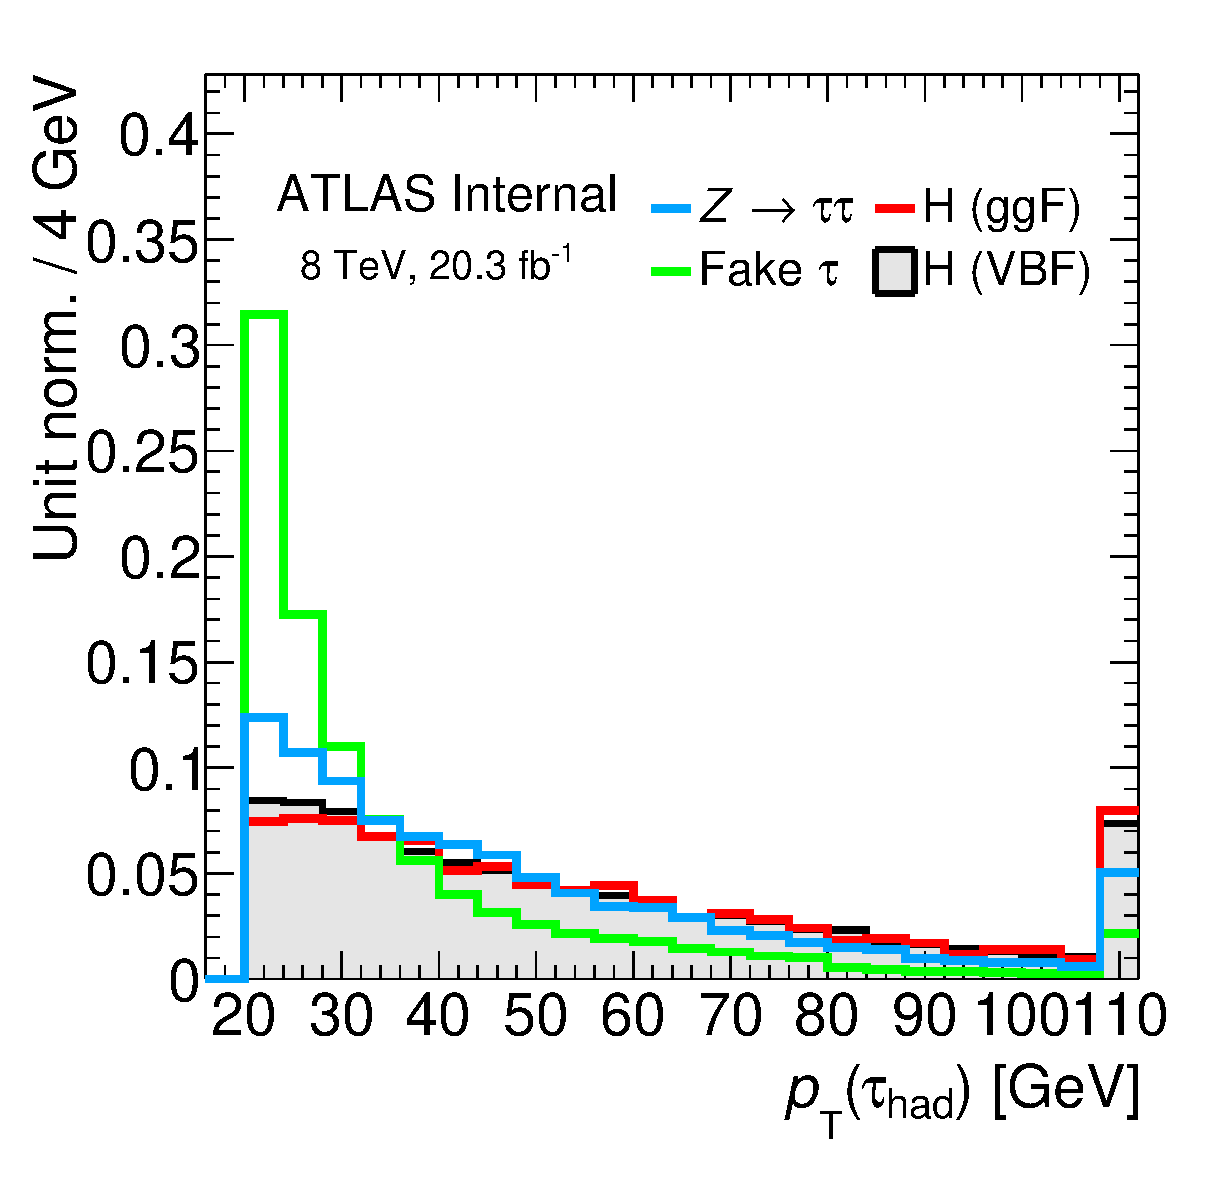
\includegraphics[width=0.35\textwidth]{figures/overlaid/boost/tau-pt}
  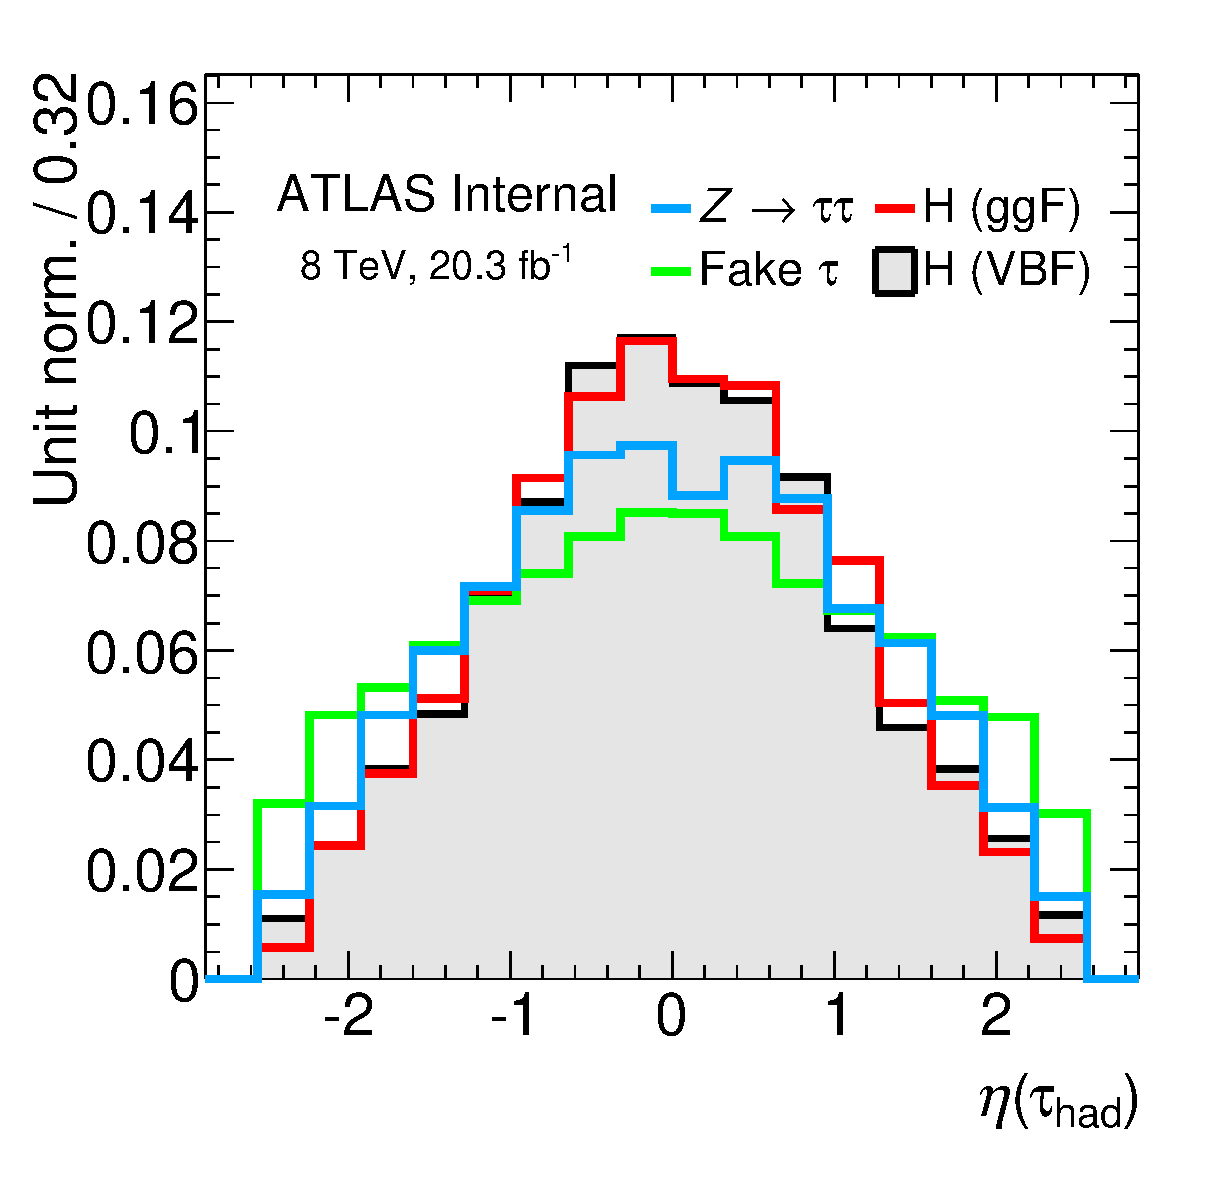
\includegraphics[width=0.35\textwidth]{figures/overlaid/boost/tau-eta}
  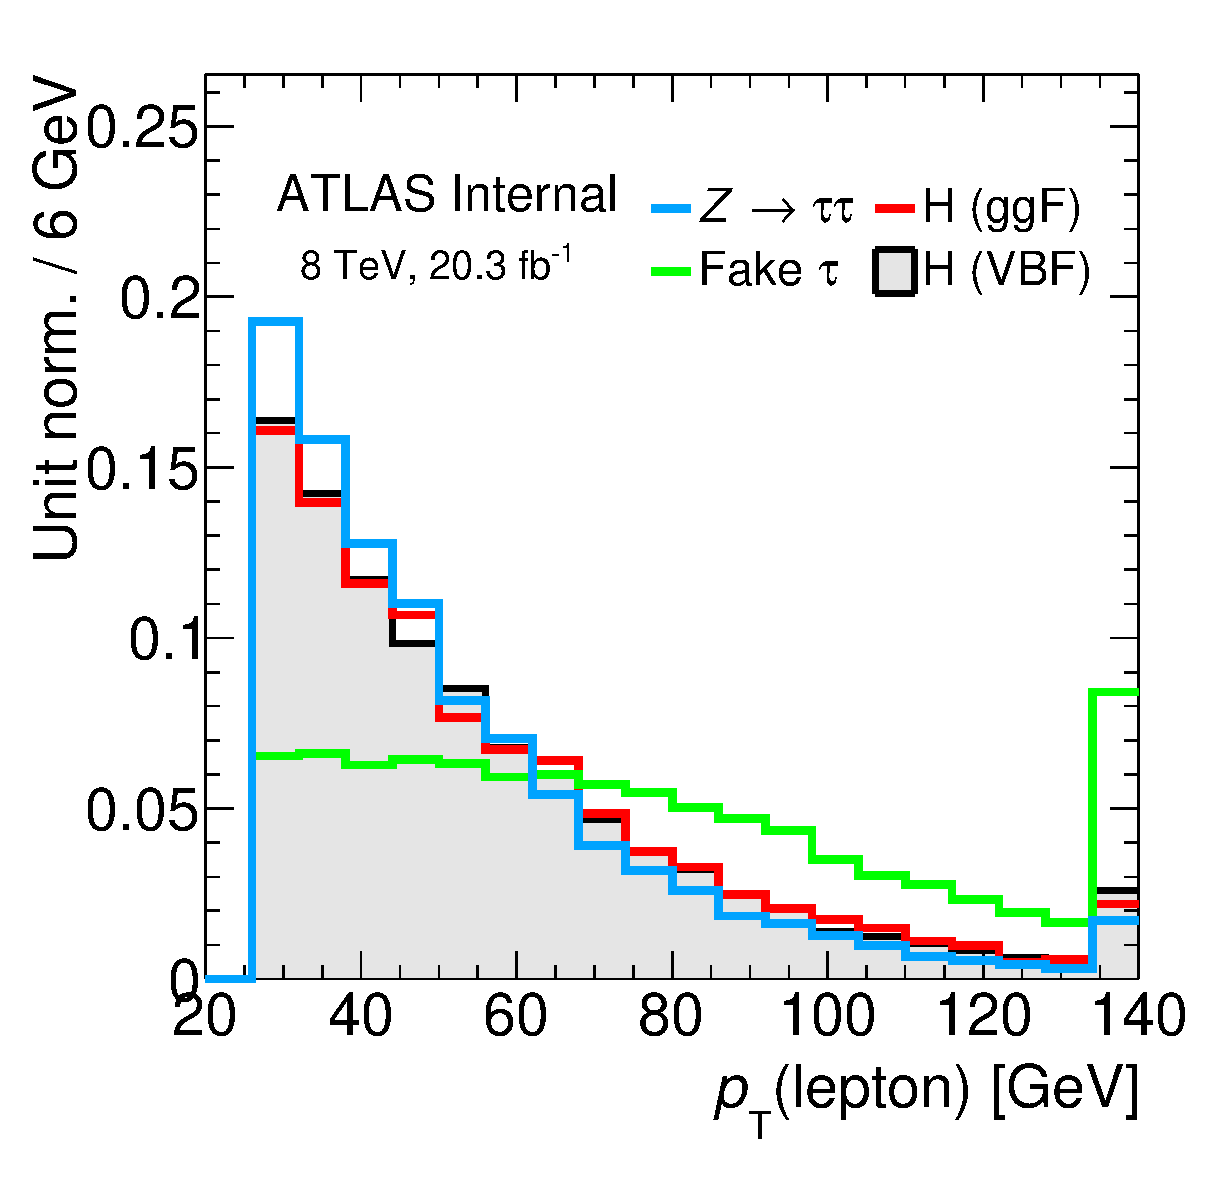
\includegraphics[width=0.35\textwidth]{figures/overlaid/boost/lep-pt-hi}
  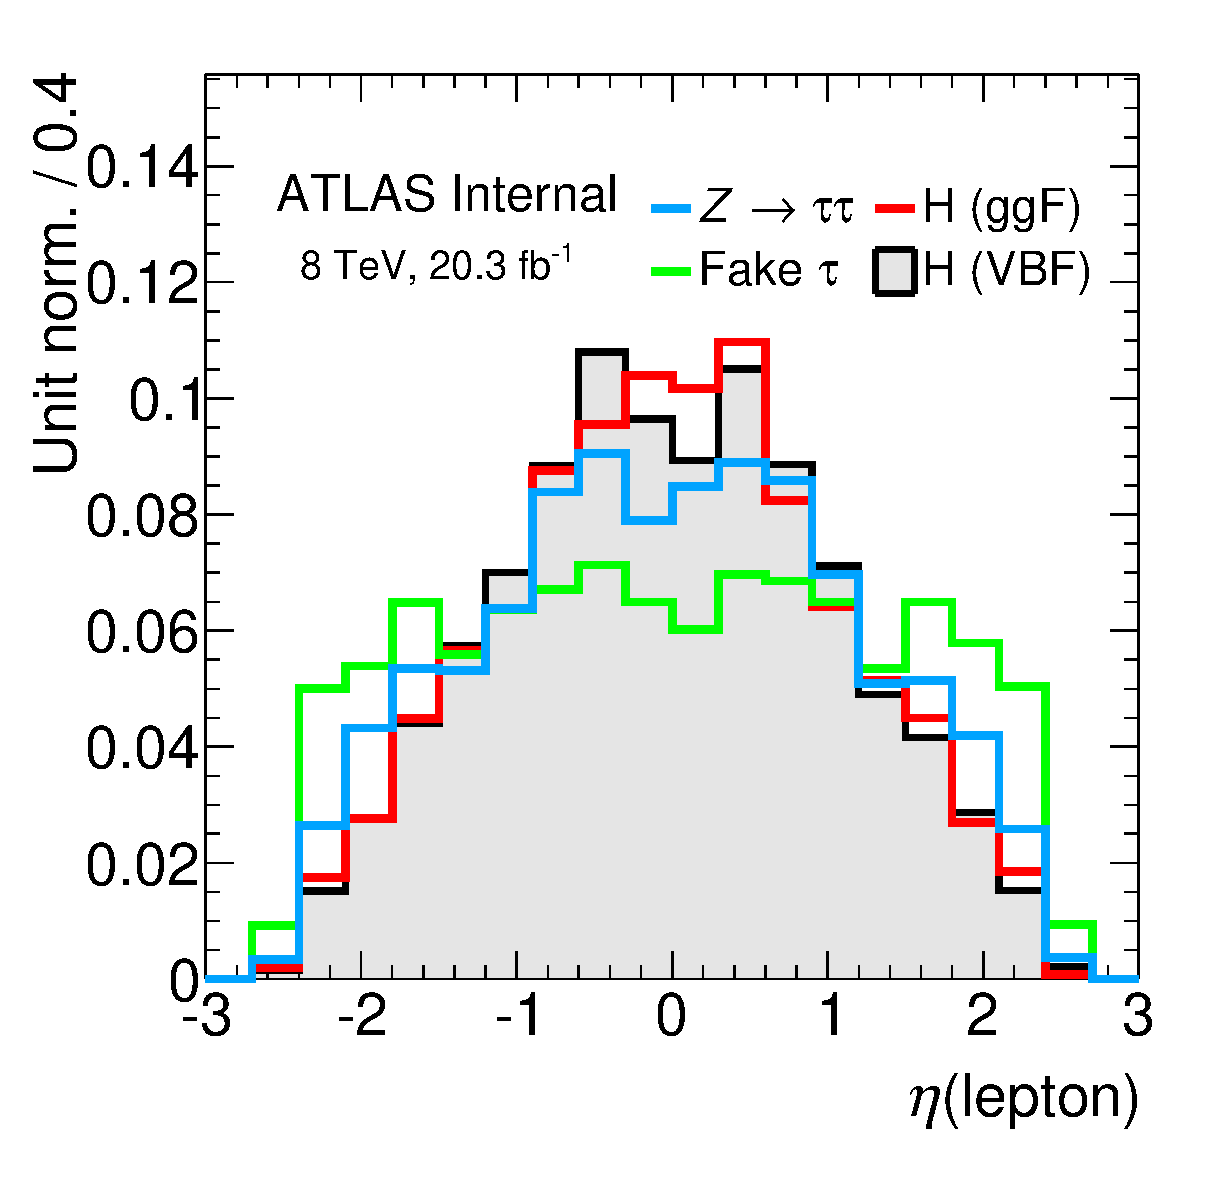
\includegraphics[width=0.35\textwidth]{figures/overlaid/boost/lep-eta}
  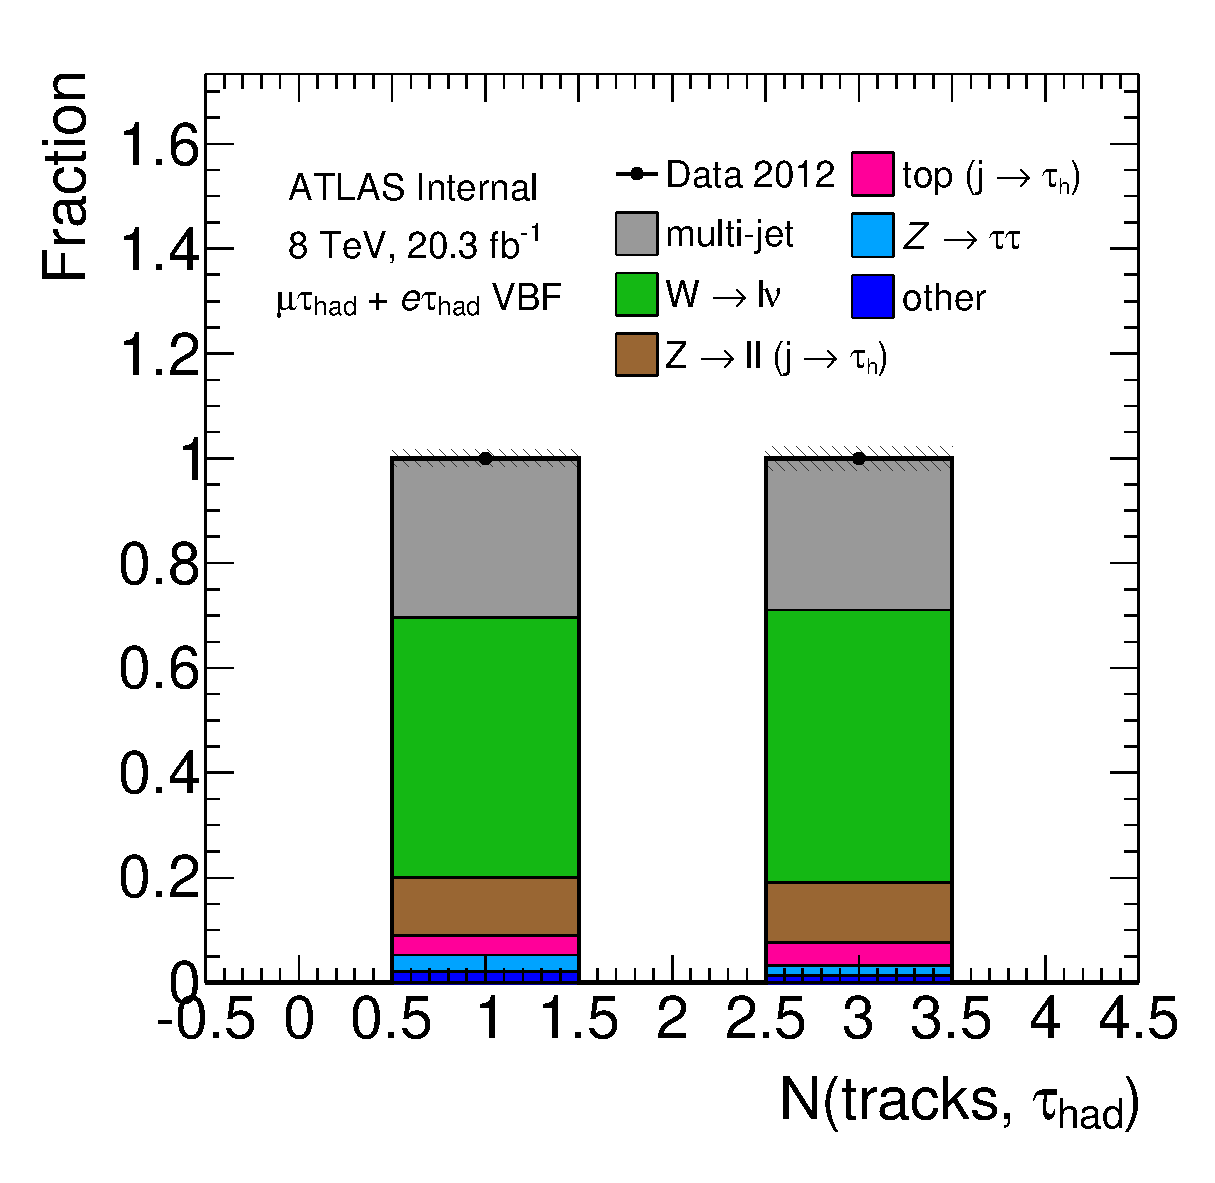
\includegraphics[width=0.35\textwidth]{figures/overlaid/boost/tau-numTrack}
  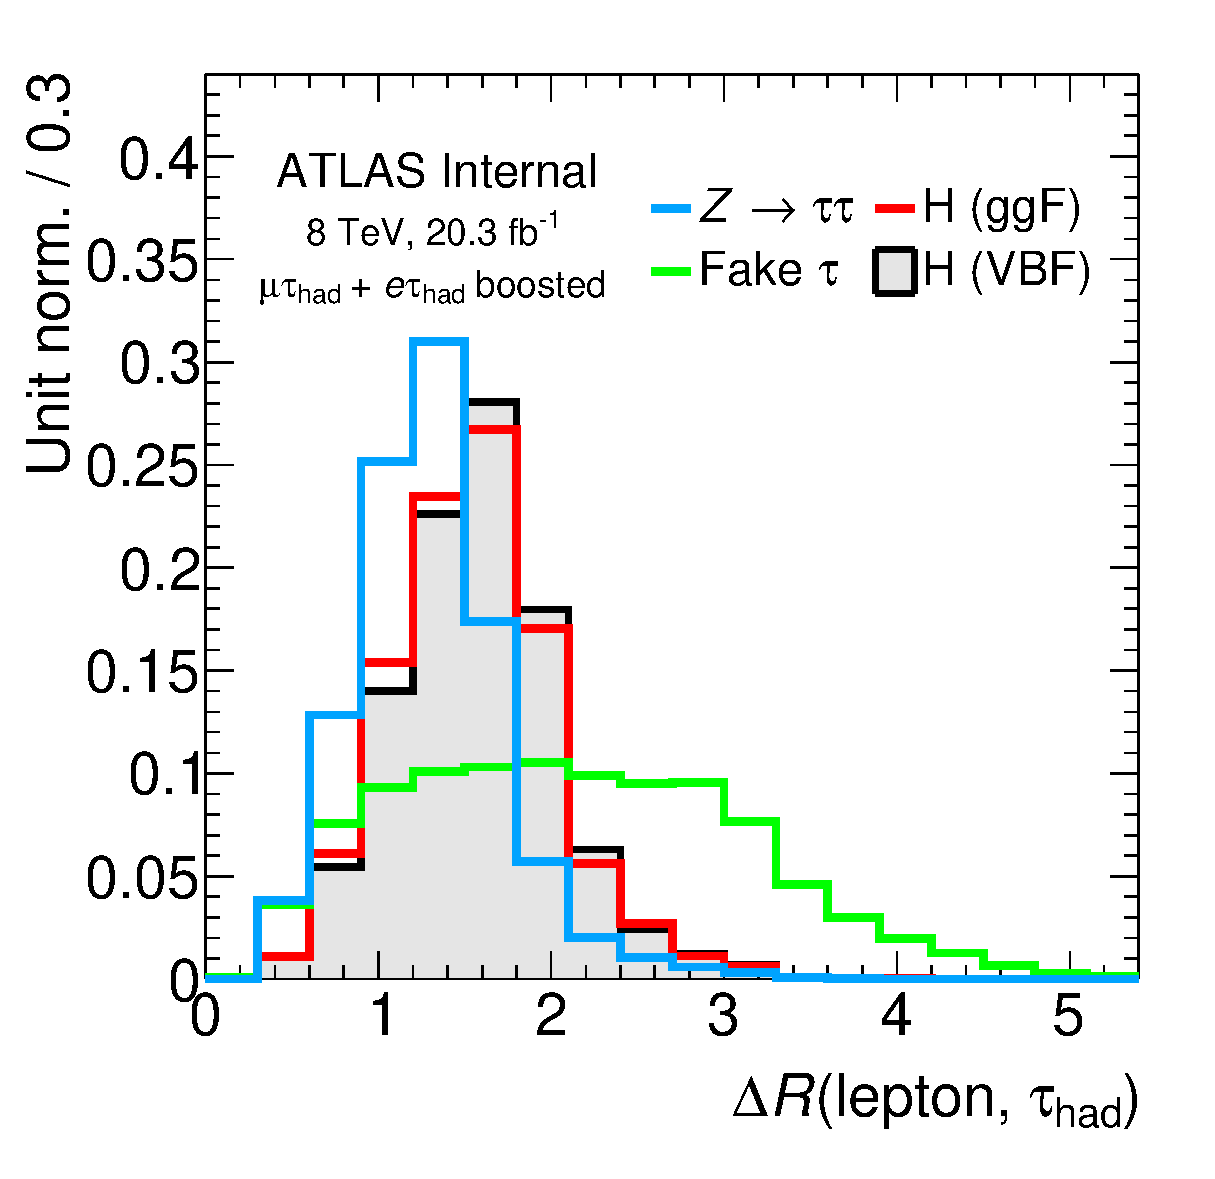
\includegraphics[width=0.35\textwidth]{figures/overlaid/boost/taulep-dR}
  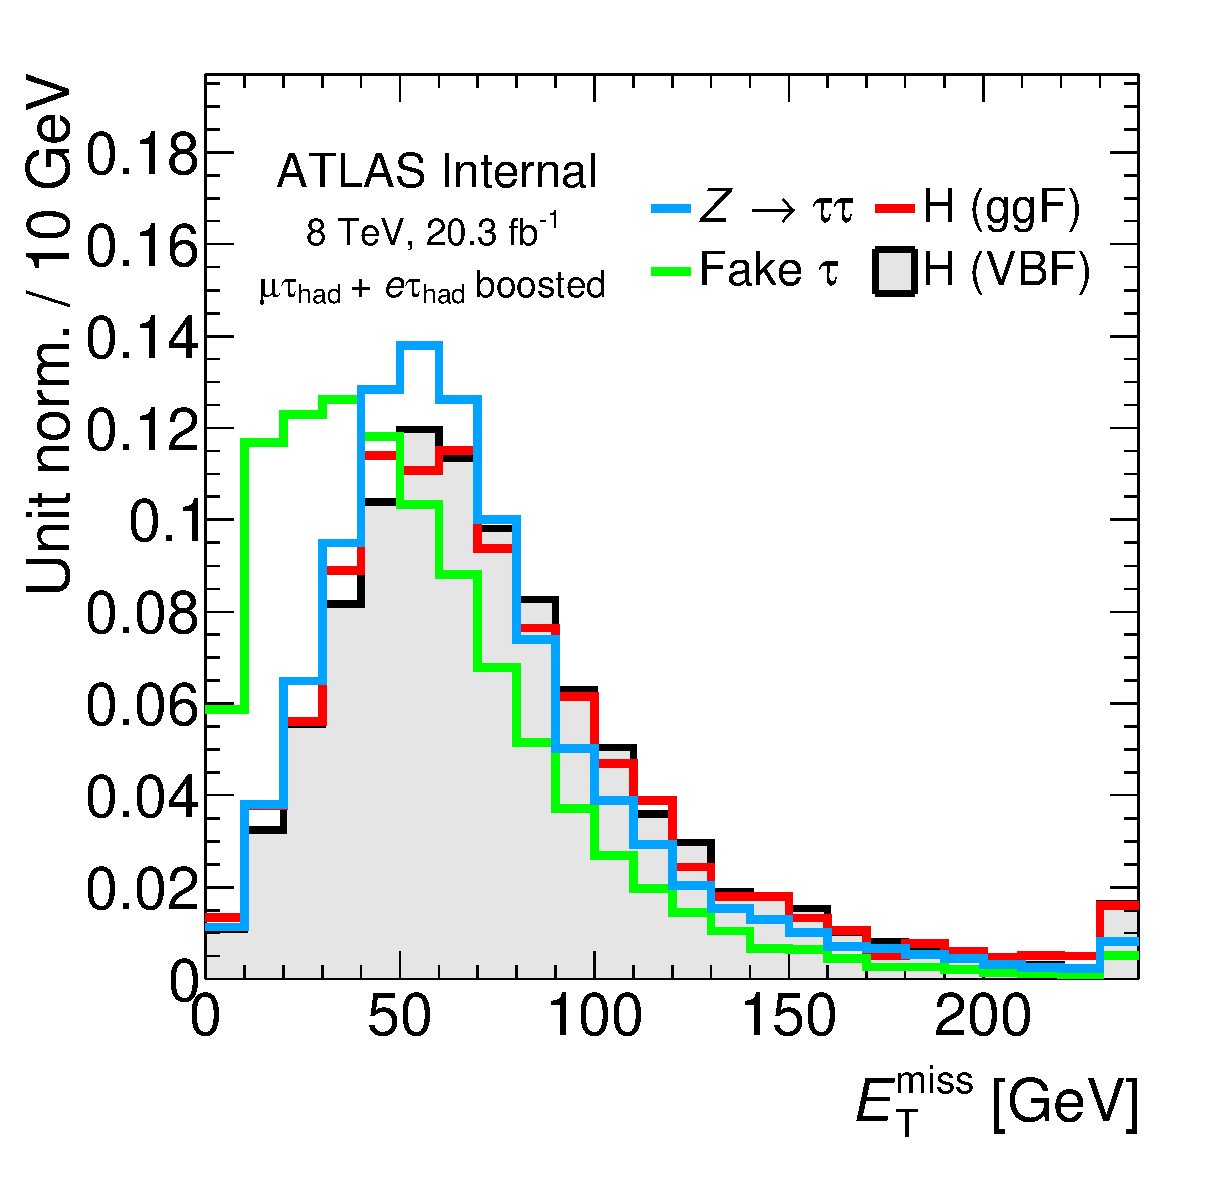
\includegraphics[width=0.35\textwidth]{figures/overlaid/boost/met-pt-hi}
  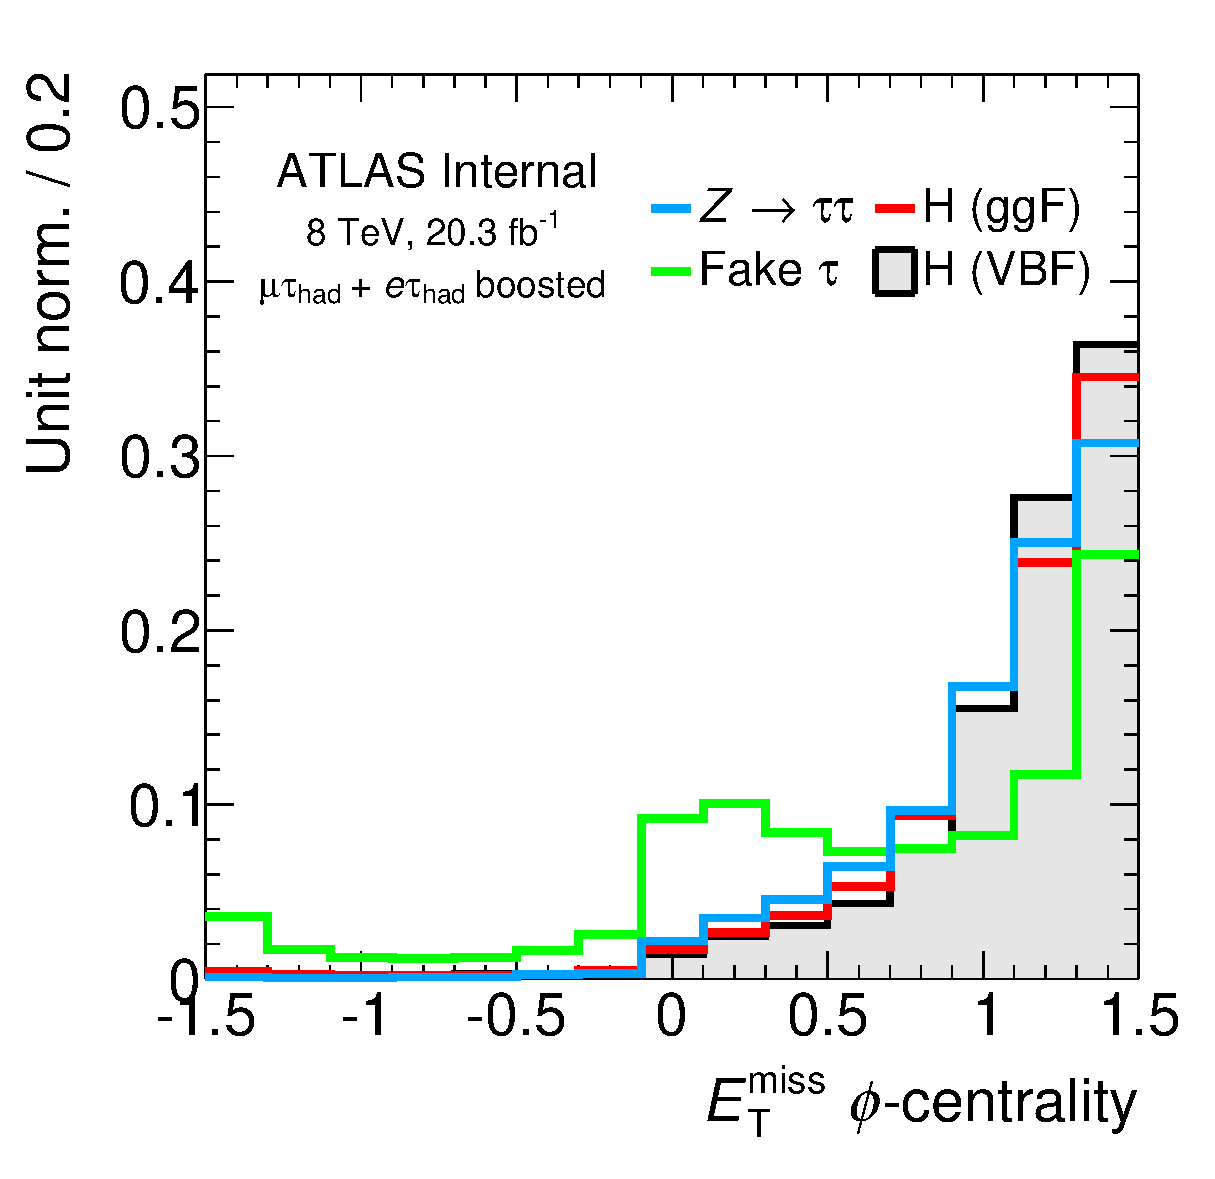
\includegraphics[width=0.35\textwidth]{figures/overlaid/boost/met-phi-centrality}
  \caption{Predicted signal and background distributions in the boosted category normalized to unit area and overlaid.}
  \label{fig:strategy-overlaid-boost-taus}
\end{figure}
\begin{figure}[tp]
  \centering
  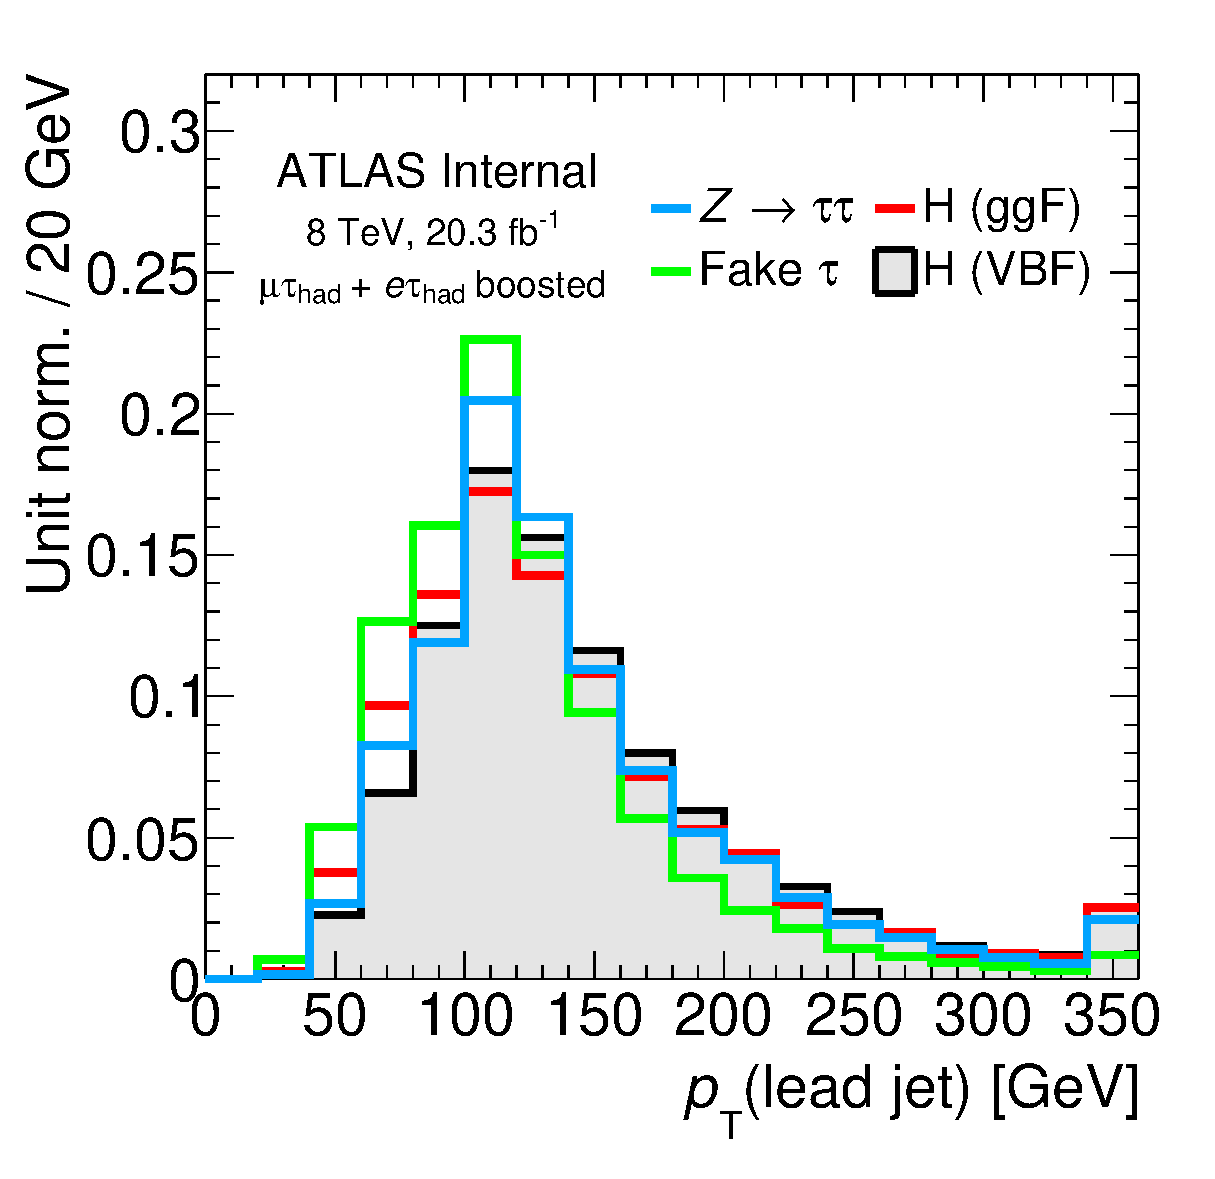
\includegraphics[width=0.45\textwidth]{figures/overlaid/boost/jet-1-pt}
  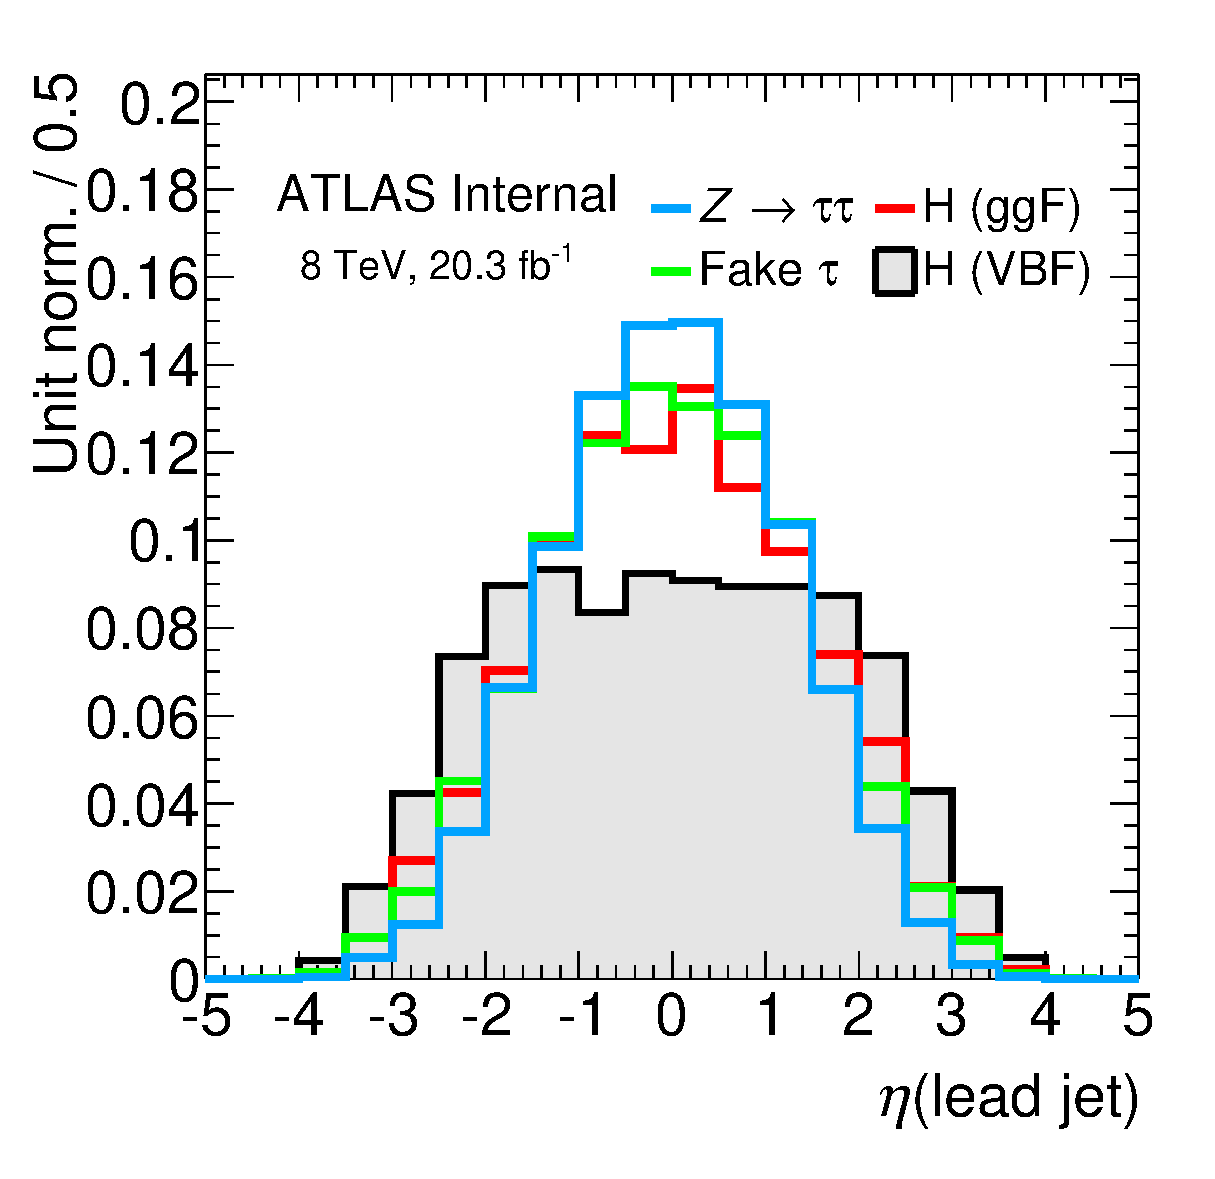
\includegraphics[width=0.45\textwidth]{figures/overlaid/boost/jet-1-eta}
  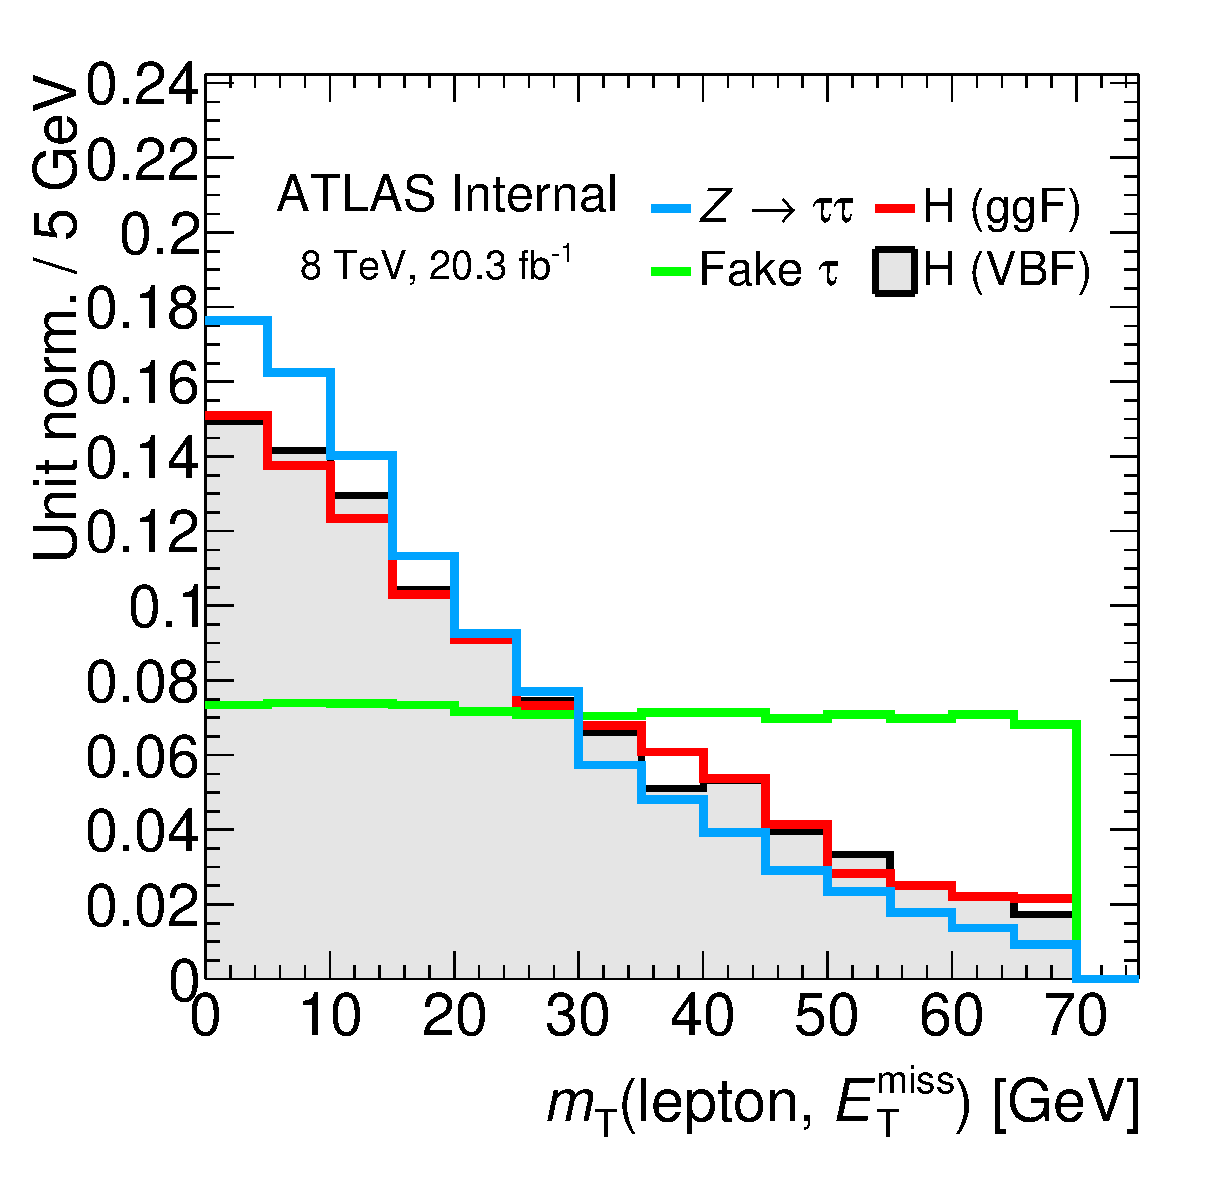
\includegraphics[width=0.45\textwidth]{figures/overlaid/boost/mT}
  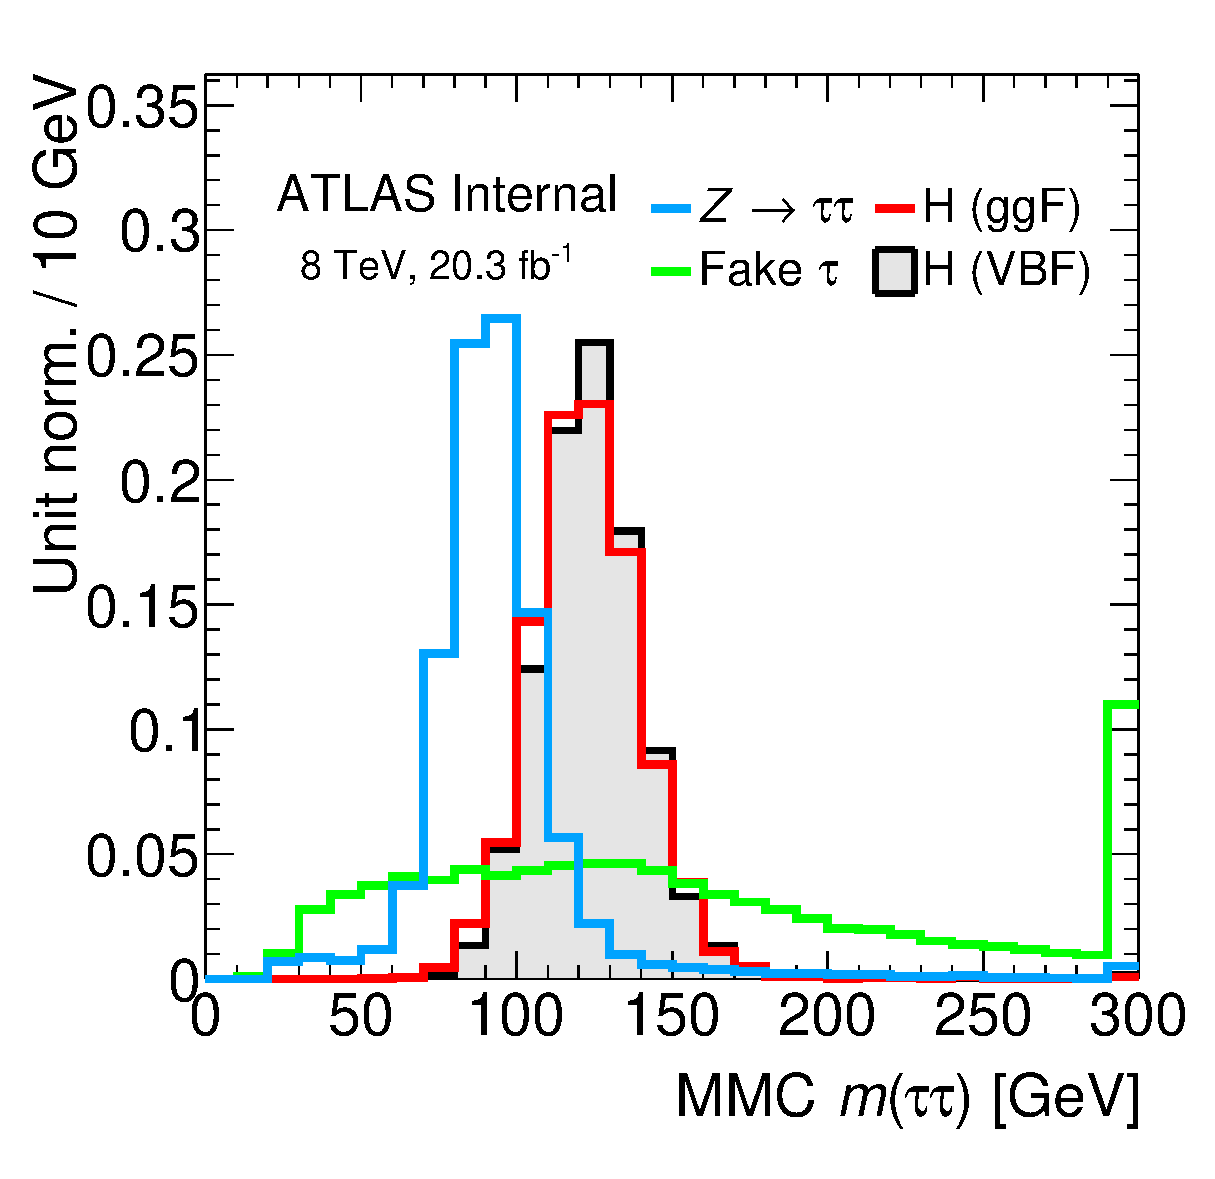
\includegraphics[width=0.45\textwidth]{figures/overlaid/boost/mMMC}
  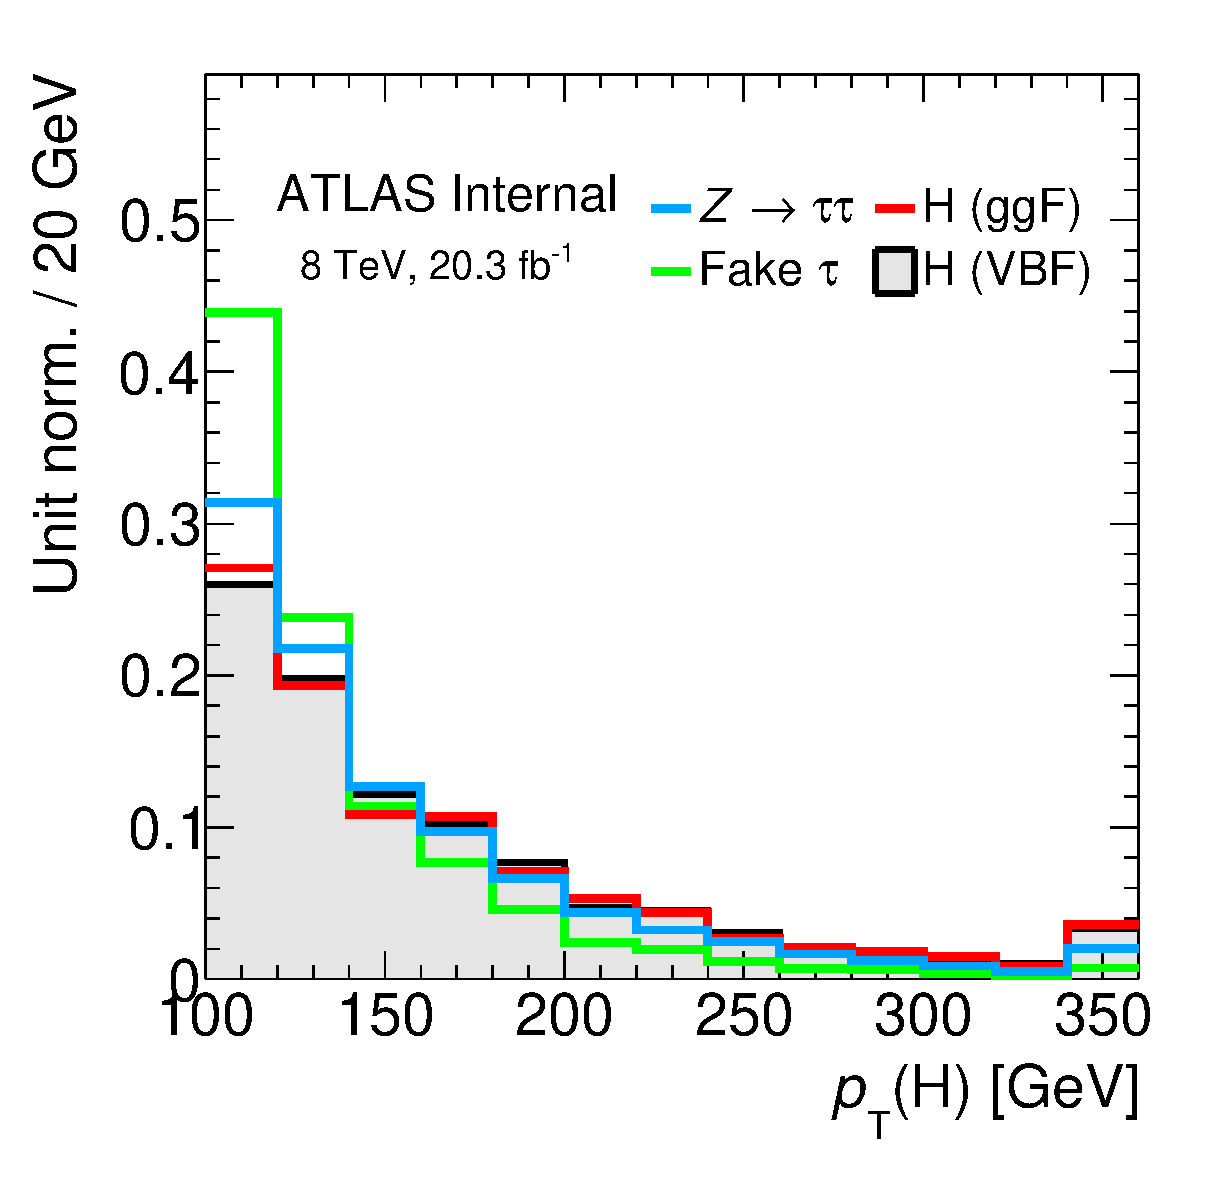
\includegraphics[width=0.45\textwidth]{figures/overlaid/boost/H-pt-hi}
  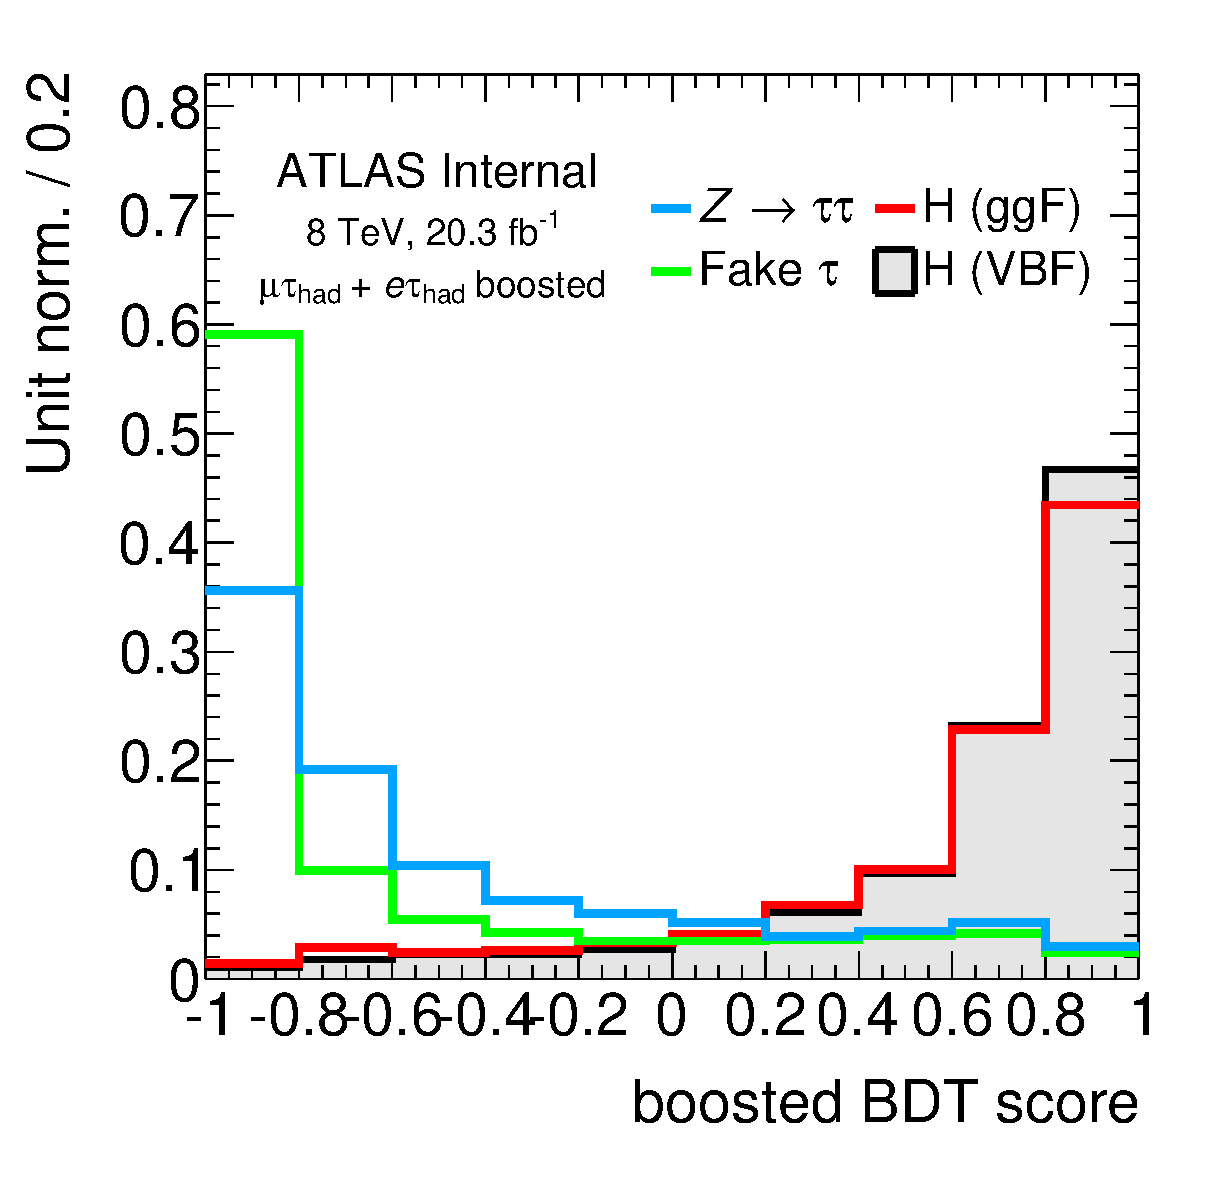
\includegraphics[width=0.45\textwidth]{figures/overlaid/boost/BDTEve-boost}
  \caption{Predicted signal and background distributions in the boosted category normalized to unit area and overlaid.}
  \label{fig:strategy-overlaid-boost-other}
\end{figure}
% ---------------------------------------------------------------------------------

% VBF
% ---------------------------------------------------------------------------------

\begin{figure}[tp]
  \centering
  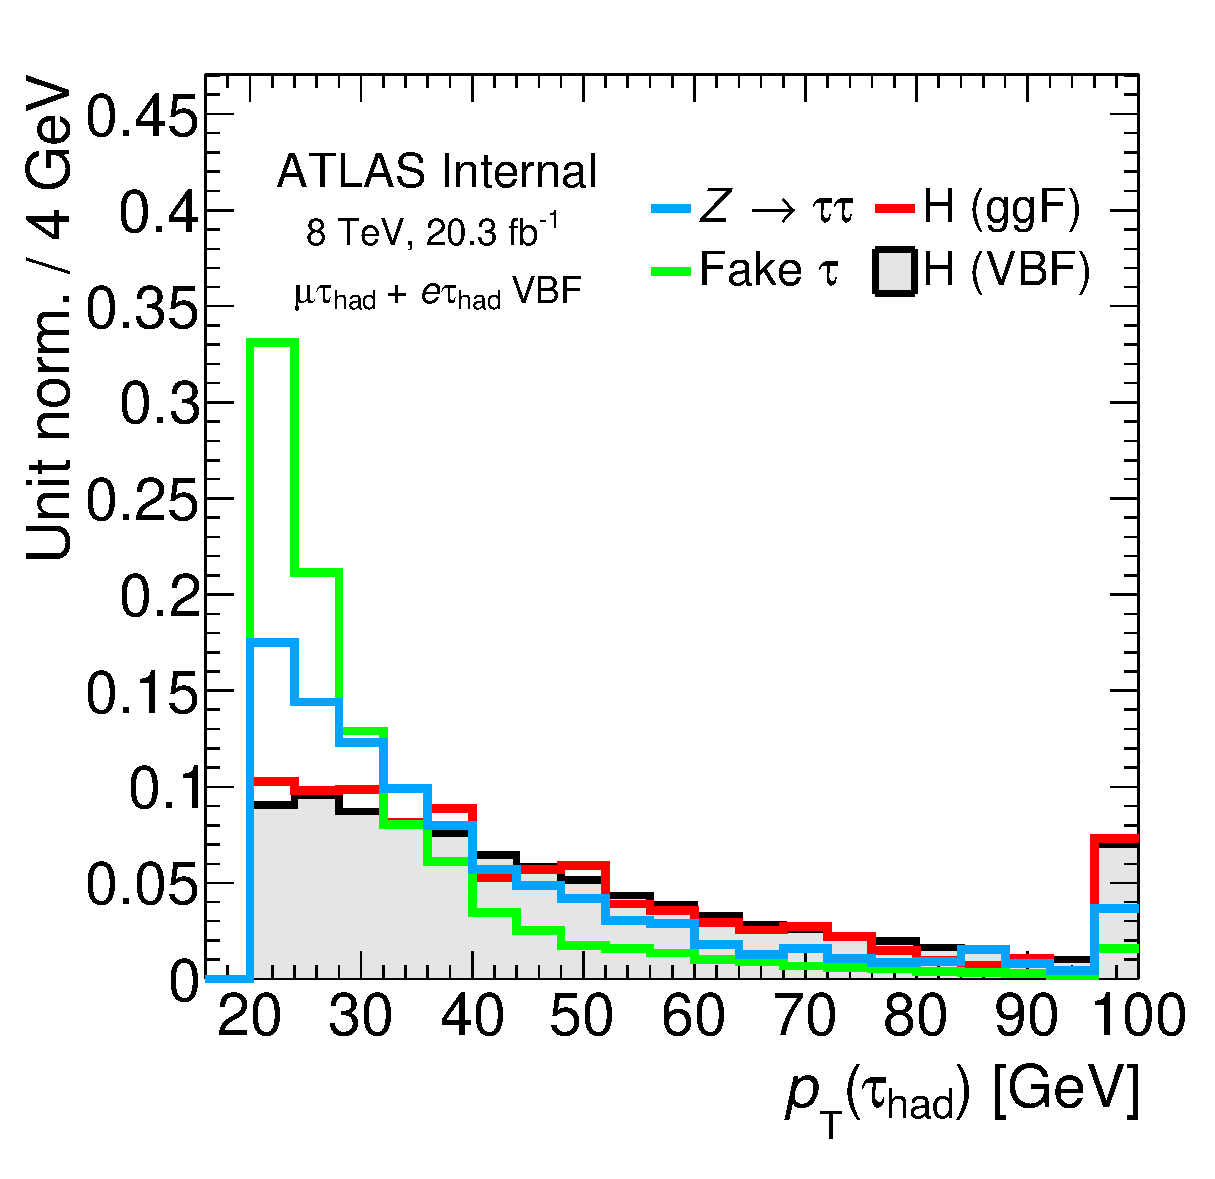
\includegraphics[width=0.35\textwidth]{figures/overlaid/vbf/tau-pt}
  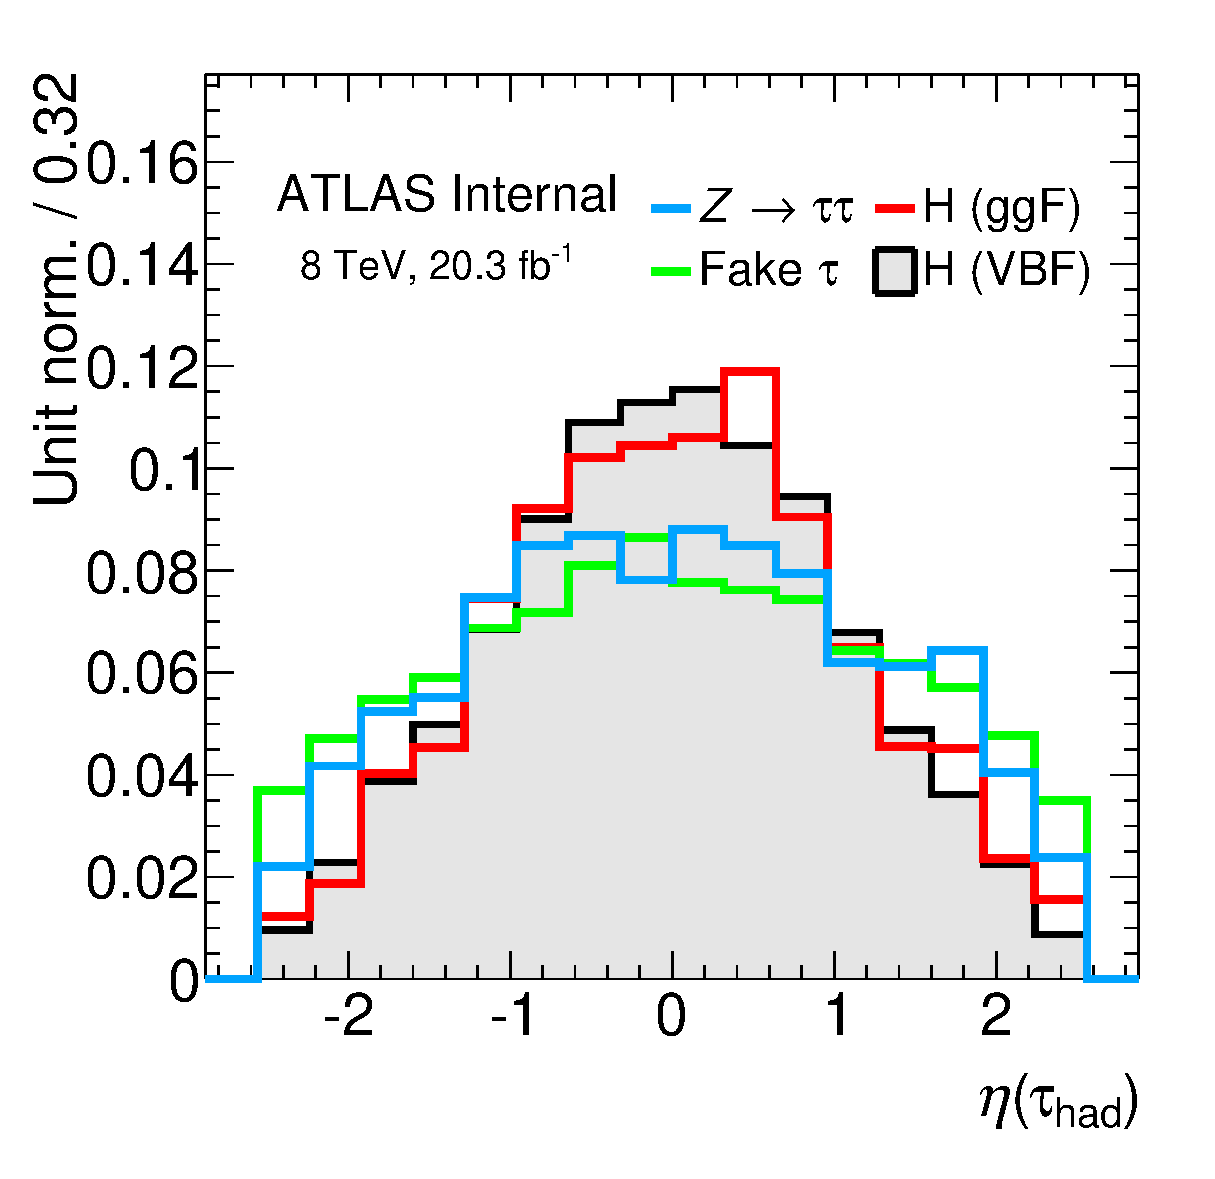
\includegraphics[width=0.35\textwidth]{figures/overlaid/vbf/tau-eta}
  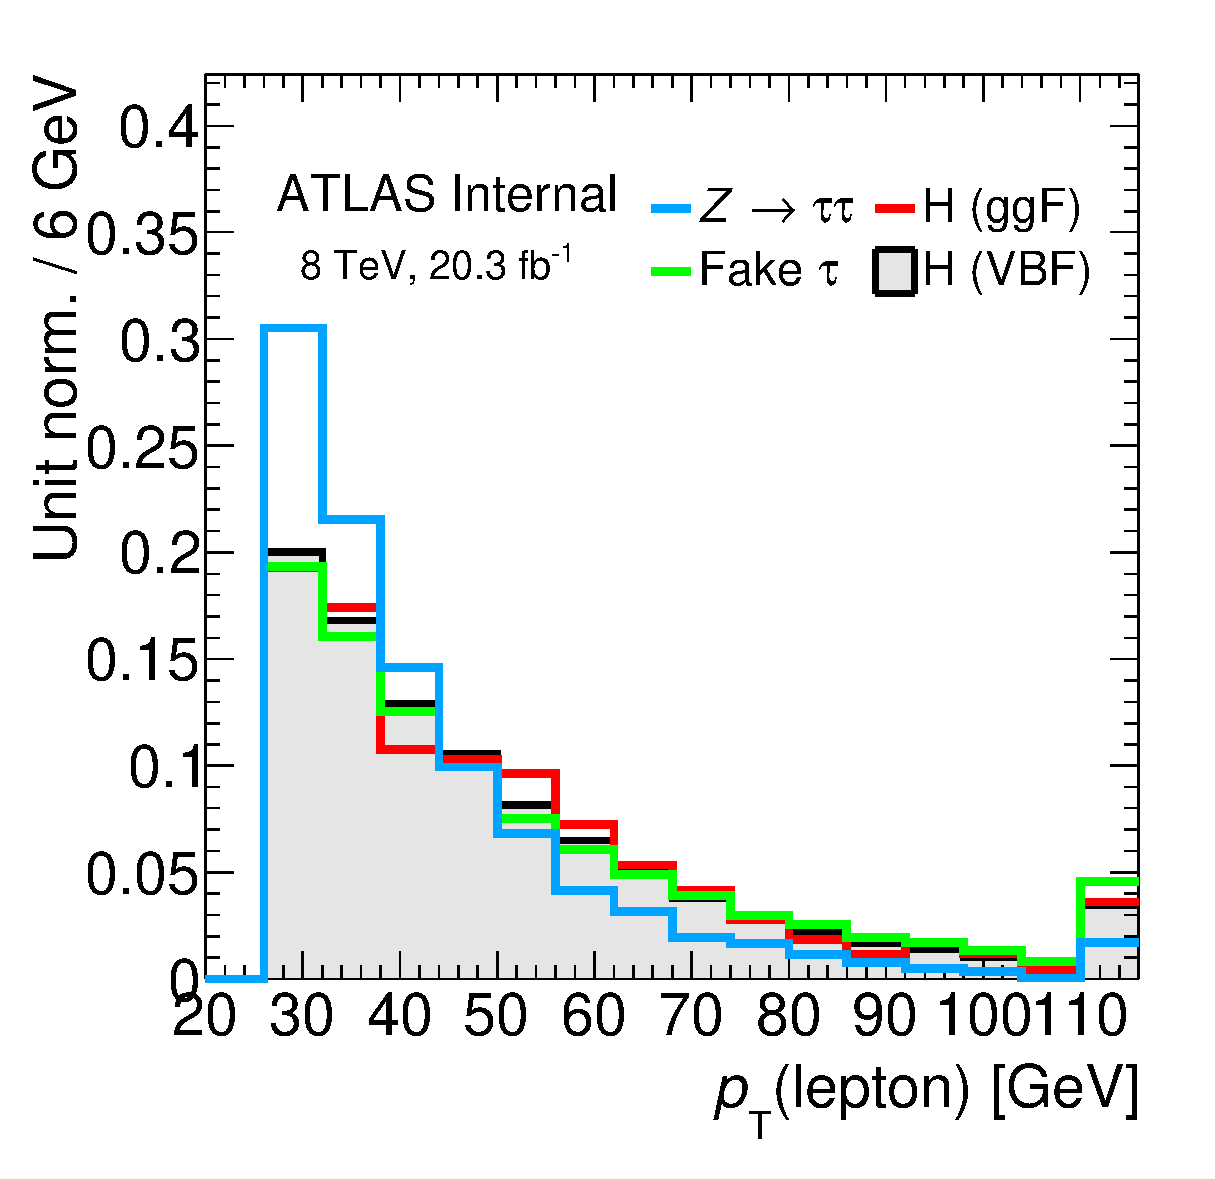
\includegraphics[width=0.35\textwidth]{figures/overlaid/vbf/lep-pt-hi}
  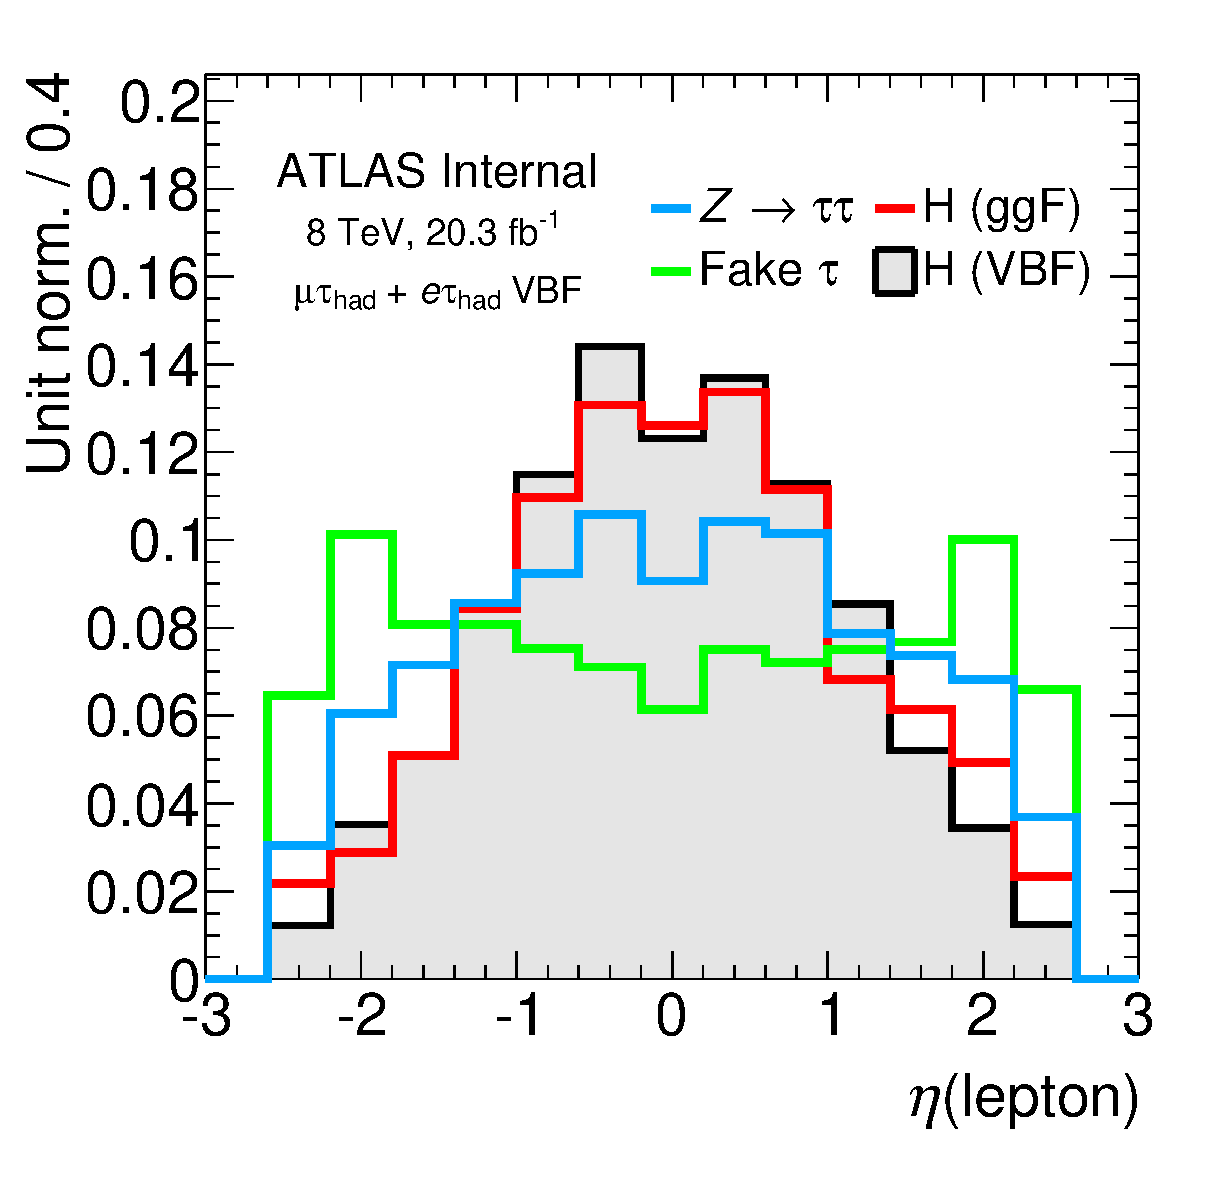
\includegraphics[width=0.35\textwidth]{figures/overlaid/vbf/lep-eta}
  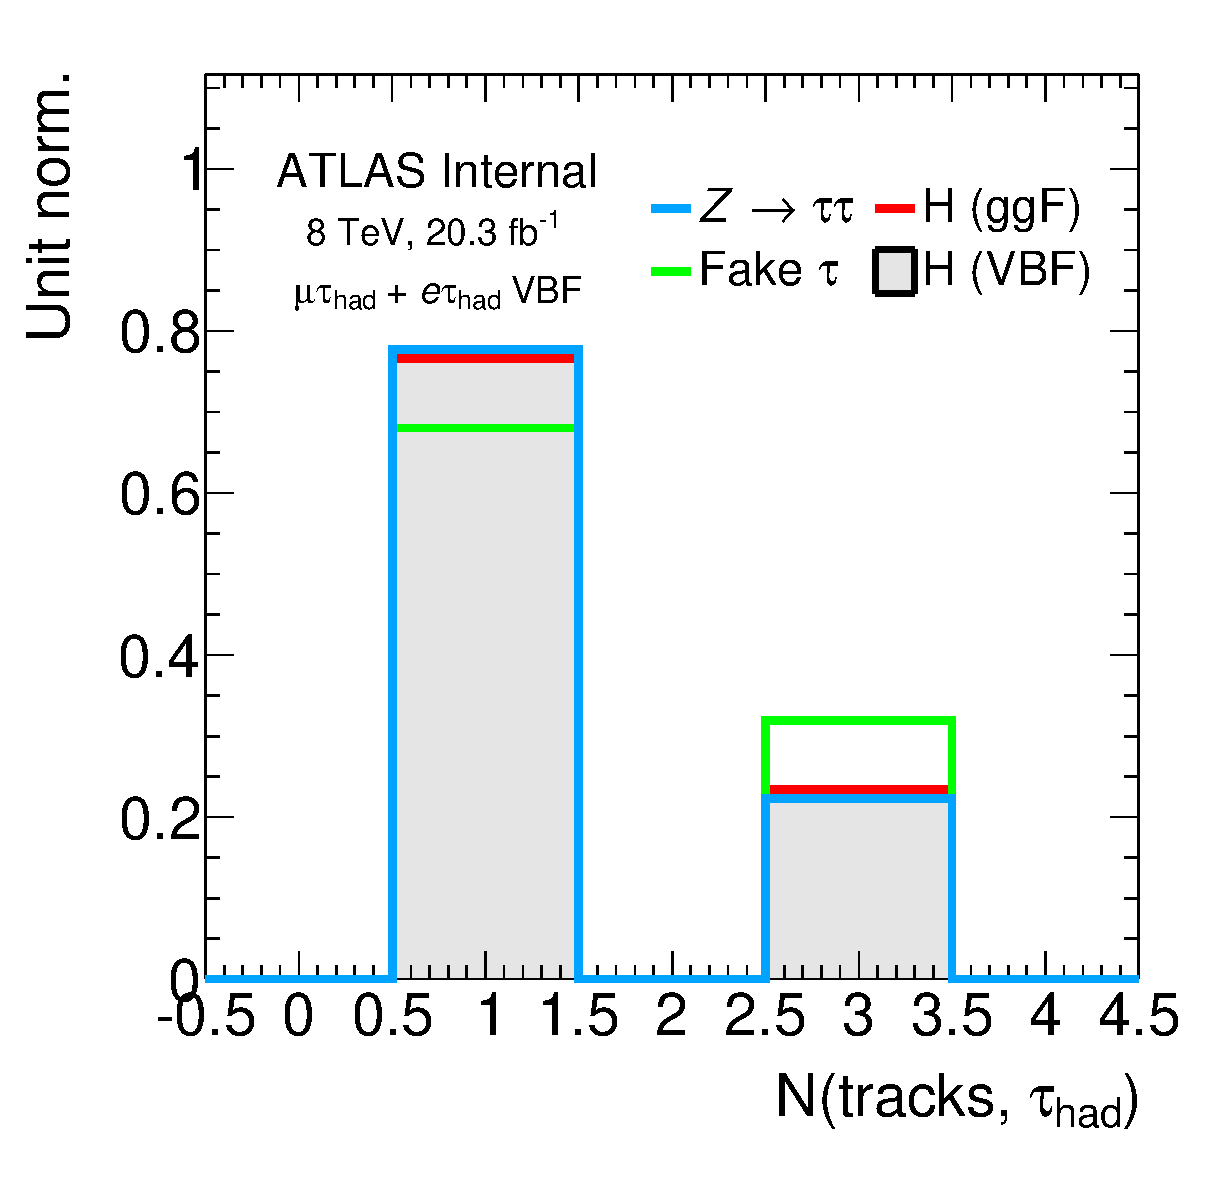
\includegraphics[width=0.35\textwidth]{figures/overlaid/vbf/tau-numTrack}
  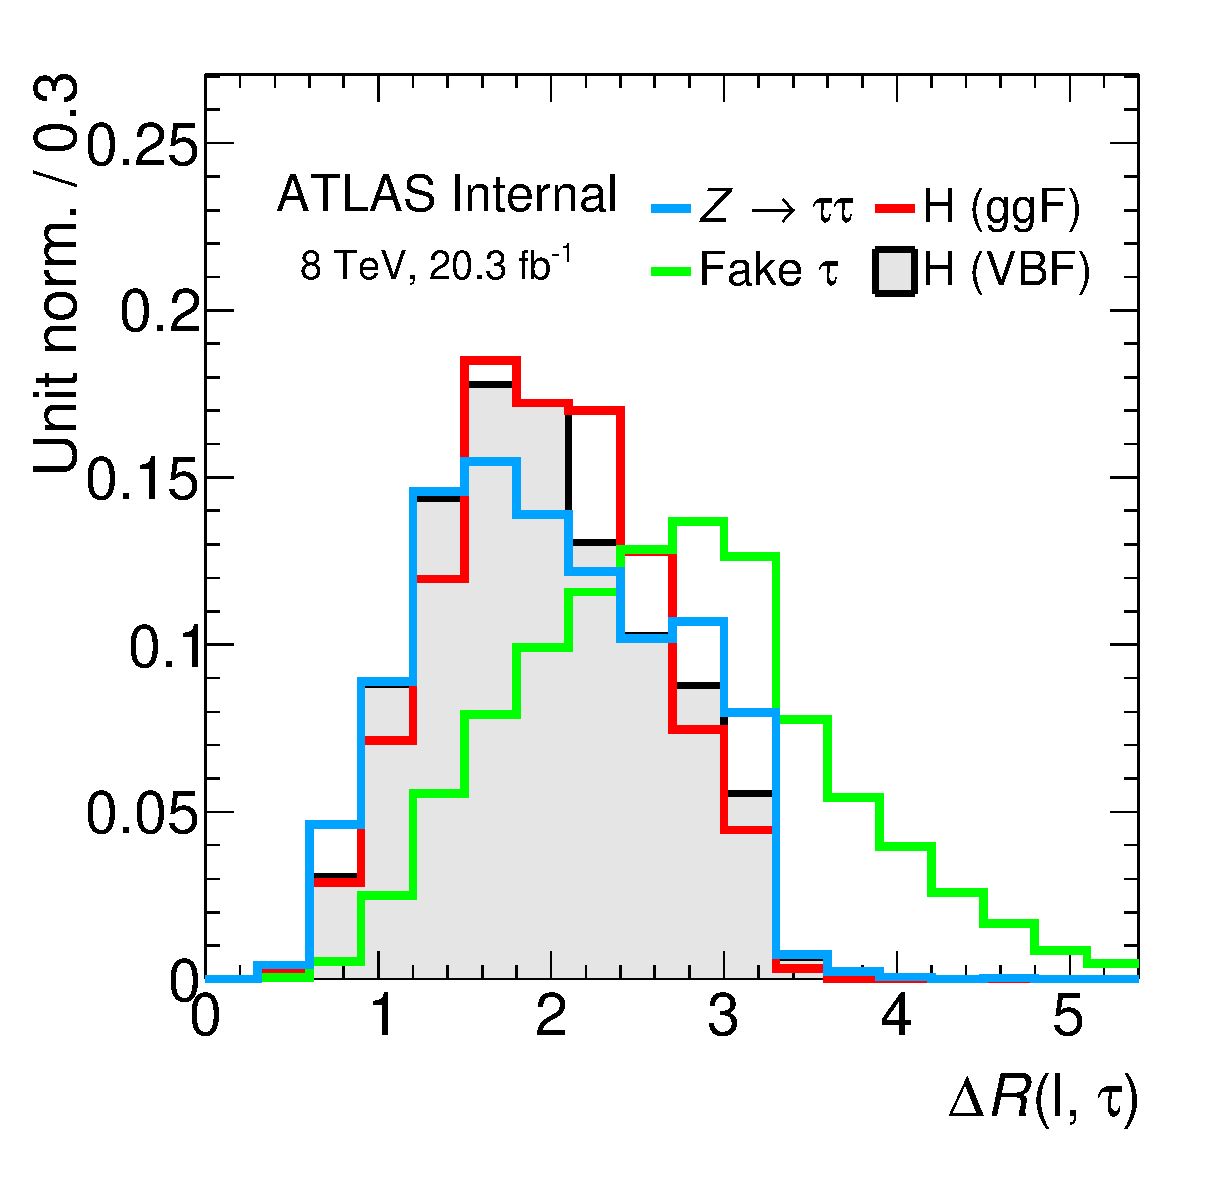
\includegraphics[width=0.35\textwidth]{figures/overlaid/vbf/taulep-dR}
  \includegraphics[width=0.35\textwidth]{figures/overlaid/vbf/met-pt-hi}
  \includegraphics[width=0.35\textwidth]{figures/overlaid/vbf/met-phi-centrality}
  \caption{Predicted signal and background distributions in the VBF category normalized to unit area and overlaid.}
  \label{fig:strategy-overlaid-vbf-taus}
\end{figure}
\begin{figure}[tp]
  \centering
  \includegraphics[width=0.35\textwidth]{figures/overlaid/vbf/jet-1-pt}
  \includegraphics[width=0.35\textwidth]{figures/overlaid/vbf/jet-1-eta}
  \includegraphics[width=0.35\textwidth]{figures/overlaid/vbf/jet-2-pt}
  \includegraphics[width=0.35\textwidth]{figures/overlaid/vbf/jet-2-eta}
  \includegraphics[width=0.35\textwidth]{figures/overlaid/vbf/dijet-m-veryhigh}
  \includegraphics[width=0.35\textwidth]{figures/overlaid/vbf/jets-deta}
  \includegraphics[width=0.35\textwidth]{figures/overlaid/vbf/jets-dphi}
  \includegraphics[width=0.35\textwidth]{figures/overlaid/vbf/jets-etaprod}
  \caption{Predicted signal and background distributions in the VBF category normalized to unit area and overlaid.}
  \label{fig:strategy-overlaid-vbf-jets}
\end{figure}
\begin{figure}[tp]
  \centering
  \includegraphics[width=0.45\textwidth]{figures/overlaid/vbf/mT}
  \includegraphics[width=0.45\textwidth]{figures/overlaid/vbf/mMMC}
  \includegraphics[width=0.45\textwidth]{figures/overlaid/vbf/H-pt-hi}
  \includegraphics[width=0.45\textwidth]{figures/overlaid/vbf/system-pt}
  \includegraphics[width=0.45\textwidth]{figures/overlaid/vbf/lep-eta-centrality}
  \includegraphics[width=0.45\textwidth]{figures/overlaid/vbf/BDTEve-VBF}
  \caption{Predicted signal and background distributions in the VBF category normalized to unit area and overlaid.}
  \label{fig:strategy-overlaid-vbf-other}
\end{figure}
% ---------------------------------------------------------------------------------

% VBF correlations
% ---------------------------------------------------------------------------------

\subsection{Correlations}
\label{sec:strategy-mva-correlations}

\clearpage

\begin{figure}[tp]
  \centering
  \includegraphics[width=0.98\textwidth]{figures/kinematiccorrelations/mT-vs-mMMC}
  \includegraphics[width=0.98\textwidth]{figures/kinematiccorrelations/taulep_dR-vs-mMMC}
  \caption{Contours of kinematic correlations in the VBF category for VBF $\Htautau$ (left), $\Ztautau$ (center), and fakes (right).}
  \label{fig:strategy-kinematic-correlations-1}
\end{figure}

\begin{figure}[tp]
  \centering
  \includegraphics[width=0.98\textwidth]{figures/kinematiccorrelations/H_pt-vs-taulep_dR}
  \includegraphics[width=0.98\textwidth]{figures/kinematiccorrelations/met_phi_cent-vs-taulep_dR}
  \caption{Contours of kinematic correlations in the VBF category for VBF $\Htautau$ (left), $\Ztautau$ (center), and fakes (right).}
  \label{fig:strategy-kinematic-correlations-2}
\end{figure}

\clearpage

\begin{figure}[tp]
  \centering
  \includegraphics[width=0.98\textwidth]{figures/kinematiccorrelations/jj_mass-vs-jj_deta}
  \includegraphics[width=0.98\textwidth]{figures/kinematiccorrelations/jj_mass-vs-jj_etaprod}
  \caption{Contours of kinematic correlations in the VBF category for VBF $\Htautau$ (left), $\Ztautau$ (center), and fakes (right).}
  \label{fig:strategy-kinematic-correlations-3}
\end{figure}

\begin{figure}[tp]
  \centering
  \includegraphics[width=0.98\textwidth]{figures/kinematiccorrelations/jj_mass-vs-mMMC}
  \includegraphics[width=0.98\textwidth]{figures/kinematiccorrelations/jj_mass-vs-taulep_dR}
  \caption{Contours of kinematic correlations in the VBF category for VBF $\Htautau$ (left), $\Ztautau$ (center), and fakes (right).}
  \label{fig:strategy-kinematic-correlations-4}
\end{figure}

\subsection{MVAs in other VBF analyses}
\label{sec:strategy-mva-elsewhere}

\begin{figure}[tp]
  \centering
  \includegraphics[width=0.32\textwidth]{figures/HIGG-2013-08/fig_06}
  \includegraphics[width=0.32\textwidth]{figures/HIGG-2013-21/fig_09f}
  \includegraphics[width=0.32\textwidth]{figures/HIGG-2013-13/fig_46a}
  \caption{Overlaid shapes of BDT outputs for signal and background processes in the VBF $\Hyy$~\cite{HIGG-2013-08}, VBF $\HZZ$~\cite{HIGG-2013-21}, and VBF $\HWW$~\cite{HIGG-2013-13} analyses.}
  \label{fig:strategy-elsewhere}
\end{figure}


